\documentclass[12pt, titlepage]{article}

\usepackage{fullpage}
\usepackage[round]{natbib}
\usepackage{multirow}
\usepackage{booktabs}
\usepackage{tabularx}
\usepackage{graphicx}
\usepackage{float}
\usepackage{xr}
\usepackage{xr-hyper}
\usepackage{hyperref}
\hypersetup{
    colorlinks,
    citecolor=blue,
    filecolor=black,
    linkcolor=red,
    urlcolor=blue
}

\usepackage{longtable}
\usepackage[utf8]{inputenc}
\usepackage{amsmath, mathtools}
\usepackage{amsfonts}
\usepackage{amssymb}
\usepackage{colortbl}
\usepackage{longtable}
\usepackage{xfrac}
\usepackage{siunitx}
\usepackage{caption}
\usepackage{pdflscape}
\usepackage{fixltx2e}
\usepackage{afterpage}
\usepackage{seqsplit}
\usepackage{underscore}
\usepackage{lscape}
\usepackage[english]{babel}
\usepackage[T1]{fontenc}
\usepackage{nameref}
\usepackage{enumitem}

%% Comments

\usepackage{color}

\newif\ifcomments\commentstrue %displays comments
%\newif\ifcomments\commentsfalse %so that comments do not display

\ifcomments
\newcommand{\authornote}[3]{\textcolor{#1}{[#3 ---#2]}}
\newcommand{\todo}[1]{\textcolor{red}{[TODO: #1]}}
\else
\newcommand{\authornote}[3]{}
\newcommand{\todo}[1]{}
\fi

\newcommand{\wss}[1]{\authornote{blue}{SS}{#1}} 
\newcommand{\plt}[1]{\authornote{magenta}{TPLT}{#1}} %For explanation of the template
\newcommand{\an}[1]{\authornote{cyan}{Author}{#1}}

%% Common Parts

\newcommand{\progname}{Mechatronics Engineering} % PUT YOUR PROGRAM NAME HERE
\newcommand{\authname}{Team \# 34, ParkingLotHawk
\\ Fady Zekry Hanna, zekryhf
\\ Winnie Trandinh, trandint
\\ Muhammad Ali, alim102
\\ Muhammad Khan, khanm120} % AUTHOR NAMES                  

\usepackage{hyperref}
    \hypersetup{colorlinks=true, linkcolor=blue, citecolor=blue, filecolor=blue,
                urlcolor=blue, unicode=false}
    \urlstyle{same}
                                

\externaldocument{../../DevelopmentPlan/DevelopmentPlan}
\externaldocument{../../HazardAnalysis/HazardAnalysis}
\externaldocument{../../SRS/SRS}
\externaldocument{../../VnVPlan/VnVPlan}
\externaldocument{../SoftDetailedDes/MIS}

\newcounter{acnum}
\newcommand{\actheacnum}{AC\theacnum}
\newcommand{\acref}[1]{AC\ref{#1}}

\newcounter{ucnum}
\newcommand{\uctheucnum}{UC\theucnum}
\newcommand{\uref}[1]{UC\ref{#1}}

\newcounter{mnum}
\newcommand{\mthemnum}{M\themnum}
\newcommand{\mref}[1]{M\ref{#1}}

\begin{document}

\title{System Design for \progname{}} 
\author{\authname}
\date{\today}

\maketitle

\pagenumbering{roman}

\section{Revision History}

\begin{tabularx}{\textwidth}{p{3cm}p{2cm}X}
\toprule {\bf Date} & {\bf Version} & {\bf Notes}\\
\midrule
January 17, 2023 & 1.0 & Initial Revision\\
\bottomrule
\end{tabularx}

\newpage

\section{Reference Material}

No external references are referenced within the System Design document.

\subsection{Abbreviations and Acronyms}

\renewcommand{\arraystretch}{1.2}
\begin{tabular}{l l} 
  \toprule		
  \textbf{symbol} & \textbf{description}\\
  \midrule 
  CAD & Computer Aided Design \\
  DMS & Degrees/Minutes/Seconds for GPS coordinates \\
  EM & Electromagnetic \\
  FR & Functional Requirements \\
  GUI & Graphical User Interface \\
  HMI & Human Machine Interface \\
  NFR & Non Functional Requirements \\
  SITL & Software in the Loop \\
  VTX & Video Transmitter \\
  \bottomrule
\end{tabular}\\

\newpage

\tableofcontents

\newpage

\listoftables

\listoffigures

\newpage

\pagenumbering{arabic}

\section{Introduction}

The System Design Document begins with defining the design goals of the ParkingLotHawk within the \nameref{sec:purpose} and \nameref{sec:scope} sections, An overview of the product and the interacting system is then provided to convey the high level system architecture of the design. The detailed design of the system components are then described within the \nameref{sec:ui}, \nameref{sec:mechHardware}, \nameref{sec:elecComponents}, and \nameref{sec:commProtocols}. The System Design Document then concludes with a proposed \nameref{sec:timeline} for the development of the ParkingLotHawk.

Further specifications of the design are defined within the  \href{https://github.com/icecap360/DroneCapstone/blob/master/docs/SRS/SRS.pdf}{SRS} and \href{https://github.com/icecap360/DroneCapstone/blob/master/docs/HazardAnalysis/HazardAnalysis.pdf}{Hazard Analysis} Document.

\section{Purpose}
\label{sec:purpose}

The System Design Document is provided in conjecture with the \href{https://github.com/icecap360/DroneCapstone/blob/master/docs/Design/SoftArchitecture/MG.pdf}{Module Guide} and \href{https://github.com/icecap360/DroneCapstone/blob/master/docs/Design/SoftDetailedDes/MIS.pdf}{Module Interface Specifications} Documents to provide a detailed system and module design of the ParkingLotHawk. This allows for transparency and traceability in design decisions for future iterations of the product. The intended audience for these documents are the project manager, development team, and project team.

\section{Scope}
\label{sec:scope}

The product, ParkingLotHawk, is an Autonomous Aerial Drone used to gather live images and data within the confines of any given outdoor parking lot. The drone records the situation of each parking space periodically, and the information is sent to the user staying on the property in a timely manner. The user of such a product is the Parking Lot Operator (called Operator for short), who communicates with the Aerial Drone using an application running on their PC.

To limit the scope of the design, the following assumptions are made:
\begin{enumerate}
    \item Operator does not fly the drone exceeding a specified amount of time, as specified by the SRS.
    \item Birds will not interfere with the drone's operation.
    \item Operator has access to a Windows computer with at least one functional USB port and Ethernet or Wifi capabilities.
    \item Parking lot lines are visible to the naked eye.
    \item Drone operates only under non-inclement weather, as defined in where \nameref{DefTable}
\end{enumerate}

The system context diagram of the product can be found in \nameref{SystemContext}.

\begin{figure}[h!]
  \begin{center} 
  \caption{System Context}
  \label{SystemContext}
        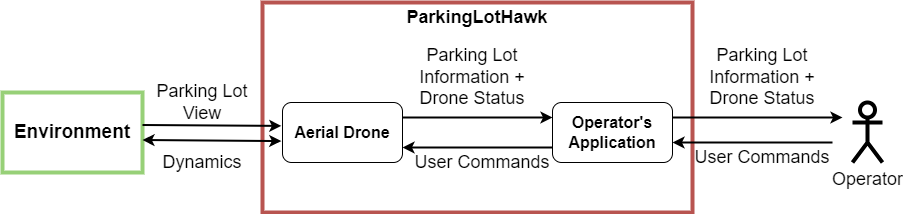
\includegraphics[width=1\textwidth]{SystemContext.png}
  \end{center}
\end{figure}

\section{Project Overview}

The product's operation can be split into two main states: \nameref{subsec:NormalBeh} and \nameref{subsec:UndesiredEvent}, which are defined in more detail within \nameref{sec:stateReqs}.

\subsection{Normal Behaviour}
\label{subsec:NormalBeh}

The following normal states are listed as per the SRS. Within this behaviour, the product shall help operators understand the parking lots and requires fully functioning hardware, software components, and communication between them. During these flight states, a c\_currentView is also outputted along with an occupancy map to the operator.

\begin{table}[!h]
\begin{center}
\caption {Normal Flight States}
\label{FlightStates}
\begin{tabular}{ | m{2.1cm} | m{3cm} | m{6cm} | m{4cm} | } 
\hline
 State & Transition Into & Behaviour & Purpose \\ 
 \hline Hover & After completion of Takeoff State. & 
    The product shall fly and hover to height i\_MaxHoverHeight. The drone shall keep the same lateral location it is currently at. The drone cannot transition to another flight state until it has reached a height of i\_MaxHoverHeight. & 
    This state is used for when the product is waiting for further operator commands. Hover height is selected to be i\_MaxHoverHeight, so that the drone can see as much of the parking lot section as it  can. \\
\hline Autonomous Move & Operator asserts m_CompulsiveMove == true and requested      location is within parking lot bounds. & 
    If the Operator requests to move to a specific location within the parking lot, the product shall move to the m\_DesiredUserLoc if it is within the parking lot, and hovers at that location with height i\_DesiredHoverHeight. Note that this height does not need to be the same as the height specified in the Hover State. & 
    This state is used for when the product needs to provide the operator the ability to move the drone to a specific location within the parking lot. \\
\hline Compulsive Move & Operator sets m_CompulsiveMove == true and requested         location is outside parking lot bounds.	& 
    If the Operator requests to move to a location, the product shall move to that location regardless of if it is within the parking lot. Once at that location, the product shall hover at a pre-defined operator-selected height. Note that this height does not need to be the same as the height specified in the Hover State.	&
    This state is used for when the product needs to provide the operator the ability to move the drone to a specific location outside of the parking lot. \\
\hline 
\end{tabular}
\end{center}
\end{table}

\begin{table}[!h]
\begin{center}
\begin{tabular}{ | m{2.1cm} | m{3cm} | m{6cm} | m{4cm} | } 
\hline
 State & Transition Into & Behaviour & Purpose \\ 
\hline Autonomous Explore & In Hover State and c_parkingLotDetected == true. & 
    The product shall create its own path to explore and remain within the parking lot it currently detects. & 
    This state is used for when the operator does not need to constantly instruct the drone to move. \\
\hline Land & m_Land == true & 
    The product shall first travel laterally to the initial launch location, and then lands vertically downward. Once physically landed, the drone enters the Idle state. & 
    This state is used to explicitly designate a landing path and command. \\
\hline Arm & In Idle state and m_Arm == true & 
    The product shall arm the motors by spinning all motors at a slow speed. & 
    This state is used to prime the motors and ensure that they are functional before liftoff. \\
\hline Takeoff & In Arm state and m_Takeoff == true & 
    During this state, the drone attempts to takeoff to i_MaxHoverHeight. & 
    This state is used to explicitly designate a takeoff procedure. \\
\hline 
\end{tabular}
\end{center}
\end{table}

\clearpage

There are also non-flight normal states, as listed in Table \ref{NonFlightStates}.

\begin{table}[!h]
\begin{center}
\caption {Non-Flight States}
\label{NonFlightStates}
\begin{tabular}{ | m{2.1cm} | m{3cm} | m{5cm} | m{5cm} | } 
\hline
 State & Transition & Behaviour & Purpose \\ 
 \hline Idle & m_PowerOn == true and the previous state was Off. & 
    The product is powered on and communicating with the operator application, but all motors are turned off.  & 
    This state is used to ensure that the operator can safely hold the drone and access the mechanical switch that controls m\_PowerOn. \\
\hline Configure & In Idle state and m_Configure == true.	& 
    During this state, the operator is able to define parameters of operation that are not configurable in other states. The Input Variables i\_MinHoverHeight, i\_MaxHoverHeight, and i\_DesiredHoverHeight can be changed in this state. The product is powered on but motors are stationary. & 
    This state is used to allow parameters that are unsafe to change during flight operation, to be safely changed through a special process. During this state the operator can safely hold the drone. \\
\hline Off & m_PowerOn == false	& 
    The product shall be unpowered and stops communication with the operator application. All modules are powered off. No battery power is consumed. c\_UserError is set to None, c\_HealthStatus is set to Healthy, and c_Connected is set to false. All values in the matrices c\_MotorSpeeds, c, c\_OccupancyMap, and c\_CurrentView are set to 0. &
    This state is used to explicitly state what it means for the drone to be off. \\
\hline 
\end{tabular}
\end{center}
\end{table}

\clearpage

\subsection{Undesired Event Handling}
\label{subsec:UndesiredEvent}

The following error states in Table \ref{ErrorStates} require no additional hardware features, and rely solely on existing functionality. Therefore, with the exception of the Malfunction state, all of the error states are guaranteed to perform correctly, even with the given error. These states are further defined within the SRS and Hazard Analysis documents.

\begin{table}[!h]
\begin{center}
\caption {Error States}
\label{ErrorStates}
\begin{tabular}{ | m{2.7cm} | m{2.3cm} | m{7.5cm} | m{2.5cm} | } 
\hline
 State & Transition & Behaviour & Purpose \\ 
 \hline Desired Location Error &
    The operator specifies an invalid desired position. & 
    Upon entry to this state, the c\_UserError variable is set to Desired\_Location\_Out\_Of\_Bounds, and set to None upon exit. The drone proceeds to Hover at its current location. Upon exit of this state, the drone shall set c\_UserError to None. Upon entry, the message "Desired Location out of parking lot bounds" shall be logged into c\_Logs. & 
    This state is used to indicate explicitly that the operator’s  request cannot be met. \\
\hline No Parking Lot Detected Error & 
    The product does not detect a valid parking lot. & 
    Upon entry to this state, the c\_UserError variable is set to No\_Lot\_Detected\_State, and while upon exit c\_UserError is set to None upon exit. The drone proceeds to Hover at its current location. Upon exit of this state, the drone shall set c\_UserError to None. Upon entry, the message "No Parking Lot detected." shall be logged into c_Logs. & 
    This state is used to indicate explicitly that the product cannot detect a parking lot. \\
\hline Malfunction & 
    An internal/external malfunction occurs in such a way that nominal performance is not possible. & 
    Upon entry, the message "Major malfunction in drone detected, please inspect" shall be added to c\_Logs. During this state the drone sets the c\_HealthStatus to Unhealthy and sets c\_HealthStatus to Healthy upon exit. It then tries to land the product at its launch location, which if is not possible the drone instead lands vertically on the land below. After landing, the drone enters the Off state. &
    This state is used to ensure that the product can handle large malfunctions that can occur during operation. \\
\hline Communication Lost & 
    The product loses connection or has a very weak connection to the Operator's Application. & 
    During this state, the drone sets the c\_HealthStatus to Unhealthy, and a message "Connection with drone lost." is sent to the Operator’s Application. Upon exit, "Connection with drone established." is logged to c\_Logs and c\_HealthStatus to Healthy. It then tries to land at its launch location and turn off. After landing the drone enters the Off state. &
    This state is used to ensure that the product can handle communication loses that can occur during operation. \\
\hline 
\end{tabular}
\end{center}
\end{table}

\clearpage

\subsection{Component Diagram}

A component diagram of the ParkingLotHawk showing the structural relations of the components can be found in Figure \ref{ComponentDiagram}.

\begin{figure}[h!]
  \begin{center} 
  \caption{Component Diagram}
  \label{ComponentDiagram}
        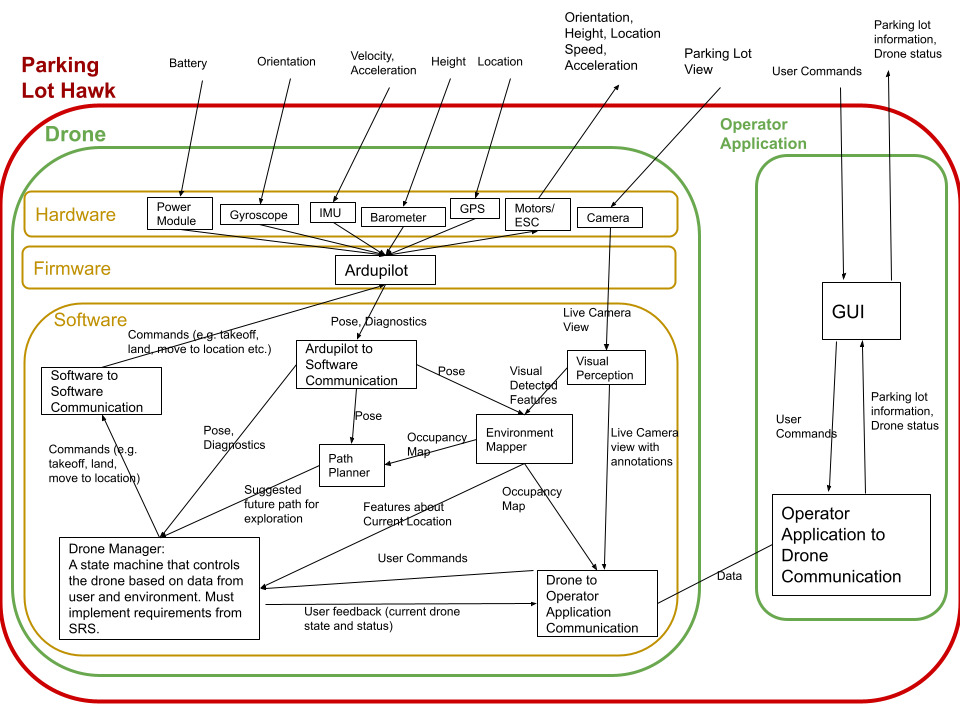
\includegraphics[width=1\textwidth]{ComponentDiagram.png}
  \end{center}
\end{figure}

\subsection{Connection Between Requirements and Design} \label{SecConnection}

The traceability matrix between the requirements within the SRS and the design components are shown within the \nameref{tab:FR_DesignTrace} and \nameref{tab:NFR_DesignTrace} for the Functional and Non-Functional requirements respectively.

\begin{table}[!h]
\begin{center}
\caption {FR Traceability Table}
\label{tab:FR_DesignTrace}
\begin{tabular}{ | m{2.5cm} | m{7.5cm} | m{7.5cm} | } 
\hline
Functional Requirement & Relevant Components & Component Reference \\
\hline
\nameref{GEN_001} & Autonomous Explore State & \nameref{FlightStates} \\ \hline
\nameref{GEN_002} & Normal Flight States & \nameref{FlightStates} \\ \hline
\nameref{GEN_003} & Configure State & \nameref{NonFlightStates} \\ \hline
\nameref{GEN_004} & Configure State & \nameref{NonFlightStates} \\ \hline
\nameref{GEN_005} & Normal Flight States & \nameref{FlightStates} \\ \hline
\nameref{GEN_006} & Normal Flight States & \nameref{FlightStates} \\ \hline
\nameref{STA_000} & Idle State & \nameref{NonFlightStates} \\ \hline
\nameref{STA_001} & Hover State & \nameref{FlightStates} \\ \hline
\nameref{STA_002} & Autonomous Move State & \nameref{FlightStates} \\ \hline
\nameref{STA_003} & Autonomous Explore State & \nameref{FlightStates} \\ \hline
\nameref{STA_004} & Configure State & \nameref{NonFlightStates} \\ \hline
\nameref{STA_005} & Off State & \nameref{NonFlightStates} \\ \hline
\nameref{STA_006} & Land State & \nameref{FlightStates} \\ \hline
\nameref{STA_007} & Desired Location Error State & \nameref{ErrorStates} \\ \hline
\nameref{STA_008} & No Parking Lot Detected Error State & \nameref{ErrorStates} \\ \hline
\nameref{STA_009} & Malfunction State & \nameref{ErrorStates} \\ \hline
\nameref{STA_010} & Communication Lost State & \nameref{ErrorStates} \\ \hline
\nameref{STA_011} & Compulsive Move State & \nameref{FlightStates} \\ \hline
\nameref{STA_012} & Arm State & \nameref{FlightStates} \\ \hline
\nameref{STA_013} & Takeoff State & \nameref{FlightStates} \\ \hline
\nameref{TRANS_001} & Off State & \nameref{FlightStates} \\ \hline
\nameref{TRANS_002} & Off State, Idle State & \nameref{NonFlightStates} \\ \hline
\nameref{TRANS_003} & Idle State, Arm State & \nameref{NonFlightStates}, \nameref{FlightStates} \\ \hline
\nameref{TRANS_004} & Hover State, Autonomous Explore State & \nameref{FlightStates} \\ \hline
\nameref{TRANS_005} & Autonomous Move State & \nameref{FlightStates} \\ \hline
\nameref{TRANS_006} & Autonomous Move State, Desired Location Error State & \nameref{FlightStates}, \nameref{ErrorStates} \\ \hline
\nameref{TRANS_007} & Autonomous Explore State & \nameref{FlightStates} \\ \hline
\nameref{TRANS_008} & Autonomous Explore State, No Parking Lot Detected Error State & \nameref{FlightStates}, \nameref{ErrorStates} \\ \hline
\nameref{TRANS_009} & Land State & \nameref{FlightStates} \\ \hline
\nameref{TRANS_010} & Communication Lost State & \nameref{ErrorStates} \\ \hline
\nameref{TRANS_011} & Communication Lost State, Hover State & \nameref{ErrorStates}, \nameref{FlightStates} \\ \hline
\nameref{TRANS_012} & Compulsive Move State & \nameref{FlightStates} \\ \hline
\nameref{TRANS_013} & Arm State, Takeoff State & \nameref{FlightStates} \\ \hline
\nameref{TRANS_014} & Takeoff State, Hover State & \nameref{FlightStates} \\ \hline
\nameref{TRANS_015} & Configure State, Idle State & \nameref{NonFlightStates} \\ \hline
\end{tabular}
\end{center}
\end{table}

\begin{table}[!h]
\begin{center}
\caption {NFR Traceability Table}
\label{tab:NFR_DesignTrace}
\begin{tabular}{ | m{2.5cm} | m{7.5cm} | m{6.5cm} | } 
\hline
Non-Functional Requirement & Relevant Components & Component Reference \\
\hline
\nameref{PERF_001} & Path Planner Module & \nameref{MIS_PATH_PLANNER} \\ \hline
\nameref{PERF_002} & Land State & \nameref{FlightStates} \\ \hline
\nameref{PERF_003} & Autonomous Move State & \nameref{FlightStates} \\ \hline
\nameref{PERF_004} & MessageSocket Module & \nameref{MIS_MESSAGE_SOCKET} \\ \hline
\nameref{PERF_005} & Hover State & \nameref{FlightStates} \\ \hline
\nameref{PERF_006} & Normal Flight States & \nameref{FlightStates} \\ \hline
\nameref{PERF_007} & All Flight States & \nameref{FlightStates}, \nameref{NonFlightStates}, \nameref{ErrorStates} \\ \hline
\nameref{PERF_008} & Autunomous Move State & \nameref{FlightStates} \\ \hline
\nameref{DES_001} & Mechanical Hardware and Electrical Components & \nameref{sec:mechHardware}, \nameref{sec:elecComponents} \\ \hline
\nameref{STD_001} & Mechanical Hardware and Electrical Components & \nameref{sec:mechHardware}, \nameref{sec:elecComponents} \\ \hline
\nameref{STD_002} & Radio Receiver & \nameref{sec:elecComponents} \\ \hline
\nameref{SEC_001} & UserInterface Module & \nameref{MIS_USER_INTERFACE} \\ \hline
\nameref{SEC_002} & UserInterface Module & \nameref{MIS_USER_INTERFACE} \\ \hline
\nameref{MTNC_001} & LiPo Battery & \nameref{sec:elecComponents} \\ \hline
\nameref{MTNC_002} & Mechanical Hardware and Electrical Components & \nameref{sec:mechHardware}, \nameref{sec:elecComponents} \\ \hline
\nameref{MTNC_003} & Mechanical Hardware & \nameref{sec:mechHardware} \\ \hline
\nameref{SAFE_001} & Flight States & \nameref{FlightStates} \\ \hline
\nameref{SAFE_002} & Configure State & \nameref{NonFlightStates} \\ \hline
\nameref{SAFE_003} & Flight States and Error States & \nameref{FlightStates}, \nameref{NonFlightStates}, \nameref{ErrorStates} \\ \hline
\nameref{SAFE_004} & Flight States and Error States & \nameref{FlightStates}, \nameref{NonFlightStates}, \nameref{ErrorStates} \\ \hline
\nameref{SAFE_005} & Mechanical Hardware & \nameref{sec:mechHardware} \\ \hline
\end{tabular}
\end{center}
\end{table}

\begin{table}[!h]
\begin{center}
\begin{tabular}{ | m{2.5cm} | m{7.5cm} | m{6.5cm} | } 
\hline
Non-Functional Requirement & Relevant Components & Component Reference \\
\hline
\nameref{USE_001} & UserInterface Module & \nameref{MIS_USER_INTERFACE} \\ \hline
\nameref{USE_002} & UserInterface Module & \nameref{MIS_USER_INTERFACE} \\ \hline
\nameref{USE_003} & Mechanical Hardware and Electrical Components & \nameref{sec:mechHardware}, \nameref{sec:elecComponents} \\ \hline
\nameref{USE_004} & UserInterface Module & \nameref{MIS_USER_INTERFACE} \\ \hline
\nameref{USE_005} & UserInterface Module & \nameref{MIS_USER_INTERFACE} \\ \hline
\nameref{SR_002} & UserInterface Module & \nameref{MIS_USER_INTERFACE} \\ \hline
\nameref{SR_003} & UserInterface Module & \nameref{MIS_USER_INTERFACE} \\ \hline
\nameref{SR_004} & Electrical Components & \nameref{sec:elecComponents} \\ \hline
\nameref{SR_005} & Electrical Components & \nameref{sec:elecComponents} \\ \hline
\nameref{SR_006} & UserInterface Module & \nameref{MIS_USER_INTERFACE} \\ \hline
\nameref{SR_007} & UserInterface Module & \nameref{MIS_USER_INTERFACE} \\ \hline
\nameref{SR_008} & Electrical Components & \nameref{sec:elecComponents} \\ \hline
\nameref{SR_009} & UserInterface Module & \nameref{MIS_USER_INTERFACE} \\ \hline
\nameref{SR_010} & UserInterface Module & \nameref{MIS_USER_INTERFACE} \\ \hline
\nameref{SR_011} & Flight States & \nameref{FlightStates} \\ \hline
\nameref{SR_012} & UserInterface Module & \nameref{MIS_USER_INTERFACE} \\ \hline
\nameref{SR_013} & UserInterface Module & \nameref{MIS_USER_INTERFACE} \\ \hline
\end{tabular}
\end{center}
\end{table}

\clearpage

\section{System Variables}

The system variables within ParkingLotHawk are split into three main categories: 
\nameref{subsec:Monitored Variables}, \nameref{subsec:Controlled Variables}, and \nameref{subsec:Constants Variables}, and are defined in their respective sections.

\subsection{Monitored Variables}
\label{subsec:Monitored Variables}

Monitored Variables are variables that are continuously monitored by the product.
\begin{table}[!h]
\begin{center}
\caption {Monitored Variables} \label{tab:MonitoredVars}
\begin{tabular}{ | m{3cm} | m{2cm} | m{2cm} | m{8cm} | } 
\hline
Variable Name & Type & Unit & Description \\ 
\hline
m\_Acceleration	& Vector& $m/s^2$ & three-dimensional vector containing acceleration relative to frame of the drone. \\
\hline
m\_Gyroscope & Vector	&Rad &	 three-dimensional vector containing orientation relative to frame of the drone.\\
\hline
m\_Gps	& Tuple &	\{DMS, m\} &	 current GPS coordinates of the drone with height in the second tuple.\\
\hline
m\_Barometer	& Float&	atm	 &Altitude detection using atmospheric pressure measurement\\
\hline
m\_DesiredUserLoc &	GPS Location& DMS &	 Desired location of the aerial drone set by user.\\
\hline
m\_Arm &	Boolean	 &  - &	Indicates if the operator desires the drone to arm.  \\
\hline
m\_Configure &	Boolean	 &  - &	Indicates if the operator desires the drone to configure height parameters.  \\
\hline
m\_Takeoff &	Boolean	 &  - &	Indicates if the operator desires the drone to takeoff.  \\
\hline
m\_AutonomousExplore &	Boolean &	 -	 &Indicates if the operator desires the drone to autonomously explore the parking lot.\\ 
\hline
m\_AutonomousMove &	Boolean &	 -	 & Indicates if the operator desires the drone to go to a specific GPS location through the Autonomous Move State.\\ 
\hline
m\_CompulsiveMove &	Boolean &	 -	 &Indicates if the operator desires the drone to go to a specific GPS location through the Compulsive Move State.\\ 
\hline
m\_PowerOn&	Boolean  &	- &	Indicates if the operator desires the drone to be On or Off.\\
\hline
m\_BatteryCapacity&	Float  &	sec &	Estimated flight time in battery remaining. \\
\hline
m\_Land&Boolean&	-&	Indicates if the operator desires the drone to land.\\
\hline
m\_SaveOutput&Boolean&	-&	Opens a dialog to save the current images and maps files in a folder.\\
\hline
 m\_CamVision &	Image&	Array of Pixels&	Latest image of the section of the parking lot currently visible to the drone.\\
\hline
m\_Connected & Boolean & - & Indicates if the drone is connected and communicating with the Operator's Application. \\
\hline
\end{tabular}
\end{center}
\end{table}

\clearpage

\subsection{Controlled Variables}
\label{subsec:Controlled Variables}

Controlled Variables are variables that are outputted by the system. Some are visible to the operator on their application, while others help to indirectly accomplish functional requirements. 

\begin{table}[!h]
\begin{center}
\caption {Controlled Variables} \label{tab:ControlVars}
\begin{tabular}{ | m{2.5cm} | m{2.5cm} | m{3cm} | m{7cm} |}
\hline
 Variable Name & Type & Unit & Description \\ 
 \hline
 c\_CurrentView &	Image &	Array of Pixels &	Live visual display of parking lot section the drone's currently sees, as well as any further annotations and text.\\
 \hline
c\_OccupancyMap &	Image &	Array of Pixels &	Map of available parking spots based on the drone’s previous paths. \\
\hline
c\_CurrentLoc & 	Tuple&	\{DMS, m\} & GPS coordinates are stored at the first index, height is stored in the second index.	Estimated longitudinal coordinate, lateral coordinate and height of the drone.\\
\hline
c\_PastLoc&	Vector &	DMS  &	Trace of the drone's location in the past 60 seconds (vector of GPS locations).\\
\hline
c\_MotorSpeeds &Vector&	   $rad/s^2$ &	 n-dimensional vector containing the motor speeds of however many motors the drone chooses to use (2 for helicopter, 4 for quadcopter, 6 for hexcopter, etc.). The vector contains speeds of each motor clockwise from front of the drone.\\
\hline
c\_Connected & Boolean &	- &	Indicates if connection between the drone and the operator's application is established\\
\hline
c\_ParkingLotDetected&	Boolean &	-&	Indicated if a parking lot is detected in the c_CurrentView.\\
\hline
c\_UserError &	Enumeration &	0 - None,
1 - Desired_Location_Out_Of_Bounds,
2 - No_Lot_Detected&	Indicates if a command the user requested is not feasible.\\
\hline
c\_HealthStatus &	Enumeration &	0 - Healthy,
1 - Unhealthy&	Indicates if the drone's mechanical and electrical state allows it to safely fly.  For example if there is mechanical damage, the value should be Unhealthy.\\
\hline
c\_Logs &	List of Strings &	- &	Contains a list of past log messages.\\
\hline
\end{tabular}
\end{center}
\end{table}

\clearpage

\subsection{Constants Variables}
\label{subsec:Constants Variables}

There are no constants required for the design. For constants in use for the Verification and Validation Plan, see \nameref{tab:symbolic_constants}.

\section{User Interfaces}
\label{sec:ui}

The user interface consists of two parts: Hardware Interface and Software Interface. The Hardware Interface will be limited in order to minimize damage to the product from improper handling, as well as decrease any technical experience required by the operator. The only Hardware Interface present is the disconnecting and reconnecting of the battery to the drone, and the mechanical On/Off switch.

The Software User Interface for ParkingLotHawk is used to control the drone from the operator’s console. It starts with a \nameref{LoginWindow} that requests for username and password. It displays an error message if the credentials do not match. Once the operator successfully logs in, the operator is presented with two windows as described below. \\

\begin{figure}[h!]
  \begin{center} 
  \caption{Login Window}
  \label{LoginWindow}
        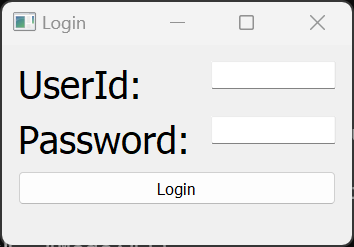
\includegraphics[width=0.35\textwidth]{MainLogin.png}
  \end{center}
\end{figure}

The first window is the \nameref{UserInterface} where the operator can view the location of the drone on the map and various information related to the drone. The information on the drone is displayed at the top of the window. There is also a logs window which displays the program status or any changes that occur in the software at the bottom. The operator can control the configurations for the drone start-up from the left section of the window. The central map displayed in the window functions similarly to the maps within SITL programs that are used for drone simulation, which is to direct the drone’s flight path from point A (drone position) to point B (drone destination) upon mouse click, and trace its movement as it moves. \\

\begin{figure}[h!]
  \begin{center} 
  \caption{User Interface}
  \label{UserInterface}
        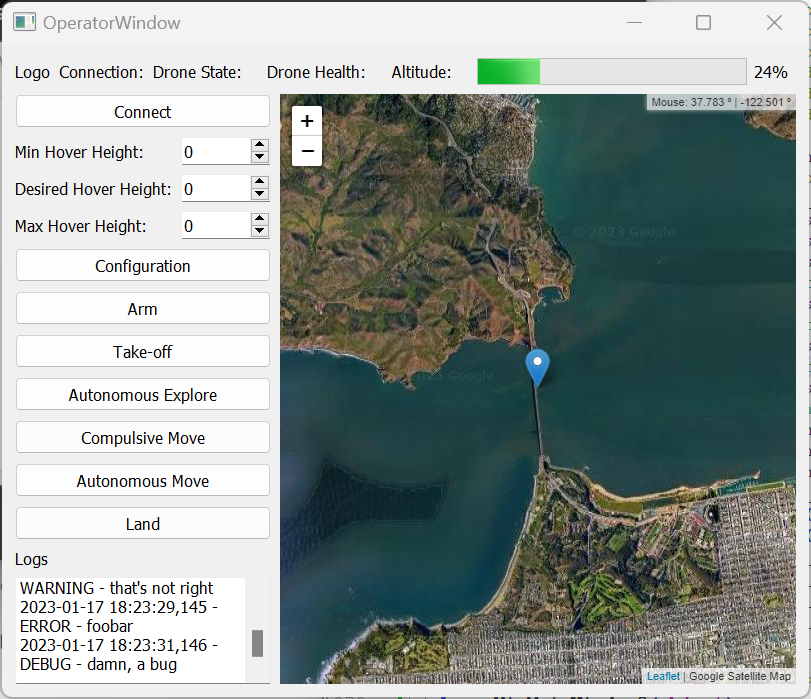
\includegraphics[width=1\textwidth]{UserInterface.png}
  \end{center}
\end{figure}

\clearpage

The second window, \nameref{CameraandOccupancy}, displays c\_currentView and the occupancy map of the entire parking lot that is currently being explored by the drone. There exists a sliding divider in the center which displays the visual images from the camera on the left and the parking lot on the right, with the status of the parking spots constantly updated by the drone. \\

\begin{figure}[h!]
  \begin{center} 
  \caption{Camera and Occupancy Map}
  \label{CameraandOccupancy}
        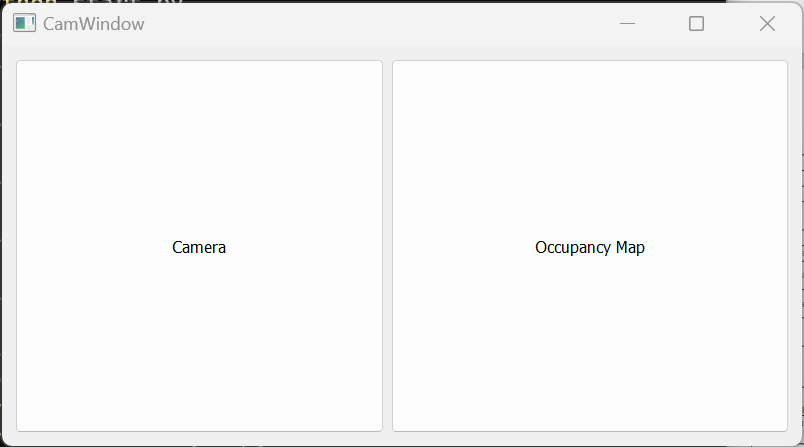
\includegraphics[width=0.65\textwidth]{CamOcc.png}
  \end{center}
\end{figure}

There are many objects that are used during the operation of the application, with the major ones being focused on in the \nameref{tab:UserInterfaceObjects} table.

\begin{table}[!h]
\begin{center}
\caption {User Interface Objects}
\label{tab:UserInterfaceObjects}
\begin{tabular}{ | m{2.5cm} | m{3.5cm} | m{2.5cm} | m{6.5cm} | } 
\hline
Name & Variable Name & Object Type & Description \\
\hline
Username & self.user_obj &  Line Textbox & Allow user to input username. \\
\hline
Password & self.user_pwd & Line Textbox & Allow user to input password. \\
\hline
Login & button_login & Button & Enable user to login and access main application. \\
\hline
Logo & self.label_1 & Label & Display Logo. \\
\hline
Connection & self.label_2 & Label & Display Wifi connection Status. \\
\hline
Drone State & self.label_3 & Label & Display the current state of the drone; whether it’s still or in motion. \\
\hline
Drone Health & self.label_4 & Label & Display any software issues or physical issues of the drone. \\
\hline
Altitude & self.label_5 & Label & Display the Drone’s altitude from the ground. \\
\hline
Battery & self.progressBar & Progress Bar & Display the drone's battery status through the progress bar. \\
\hline
Logs & self.textEdit & Textbox & Display the logs sent from the drone within a certain interval within the logs textbox. \\
\hline
Minimum Hover Height & self.spinBox_1 & Spin Box & Adjust the minimum hover height for the drone using the spinbox. \\
\hline
Desired Hover Height & self.spinBox_2 & Spin Box & Adjust the desired hover height for the drone using the spinbox. \\
\hline
Maximum Hover Height & self.spinBox_3 & Spin Box & Adjust the maximum hover height for the drone using the spinbox. \\
\hline
Connect & self.pushButton_1 & Button & Click to connect to the drone. \\
\hline
Configuration & self.pushButton_2a & Button & Click to configure drone height. \\
\hline
Take-off & self.pushButton_2b & Button & Click to Launch the drone. \\
\hline
Arm & self.pushButton_3 & Button & Click to startup the drone. \\
\hline
Autonomous Explore & self.pushButton_4 & Button & Click to automatically explore from the drone within the surroundings. \\
\hline
Compulsive Move & self.pushButton_5 & Button & Click for allowing user to control the  drone’s movement. \\
\hline
\end{tabular}
\end{center}
\end{table}

\begin{table}[!h]
\begin{center}
\begin{tabular}{ | m{2.5cm} | m{3.5cm} | m{2.5cm} | m{6.5cm} | } 
\hline
Name & Variable Name & Object Type & Description \\
\hline
Autonomous Move & self.pushButton_6 & Button & Click to have the drone move automatically. \\
\hline
Land & self.pushButton_7 & Button & Click to land the drone. \\
\hline
Map & self.webView & Web Engine Widget & Displays an online map that should have the ability to interact with the movement path of the drone. \\
\hline
Camera & -- & Input & Display the visuals from the camera mounted in the drone. \\
\hline
Occupancy Map & -- & Input & Display the status of the parking spots within the parking lot through the drone. \\
\hline
\end{tabular}
\end{center}
\end{table}

\clearpage

\section{Design of Hardware}
\label{sec:mechHardware}

The overall Computer Aided Design (CAD) of the product is shown within Figure \ref{OverallCAD}. 

\begin{figure}[h!]
  \begin{center} 
  \caption{CAD Overview}
  \label{OverallCAD}
        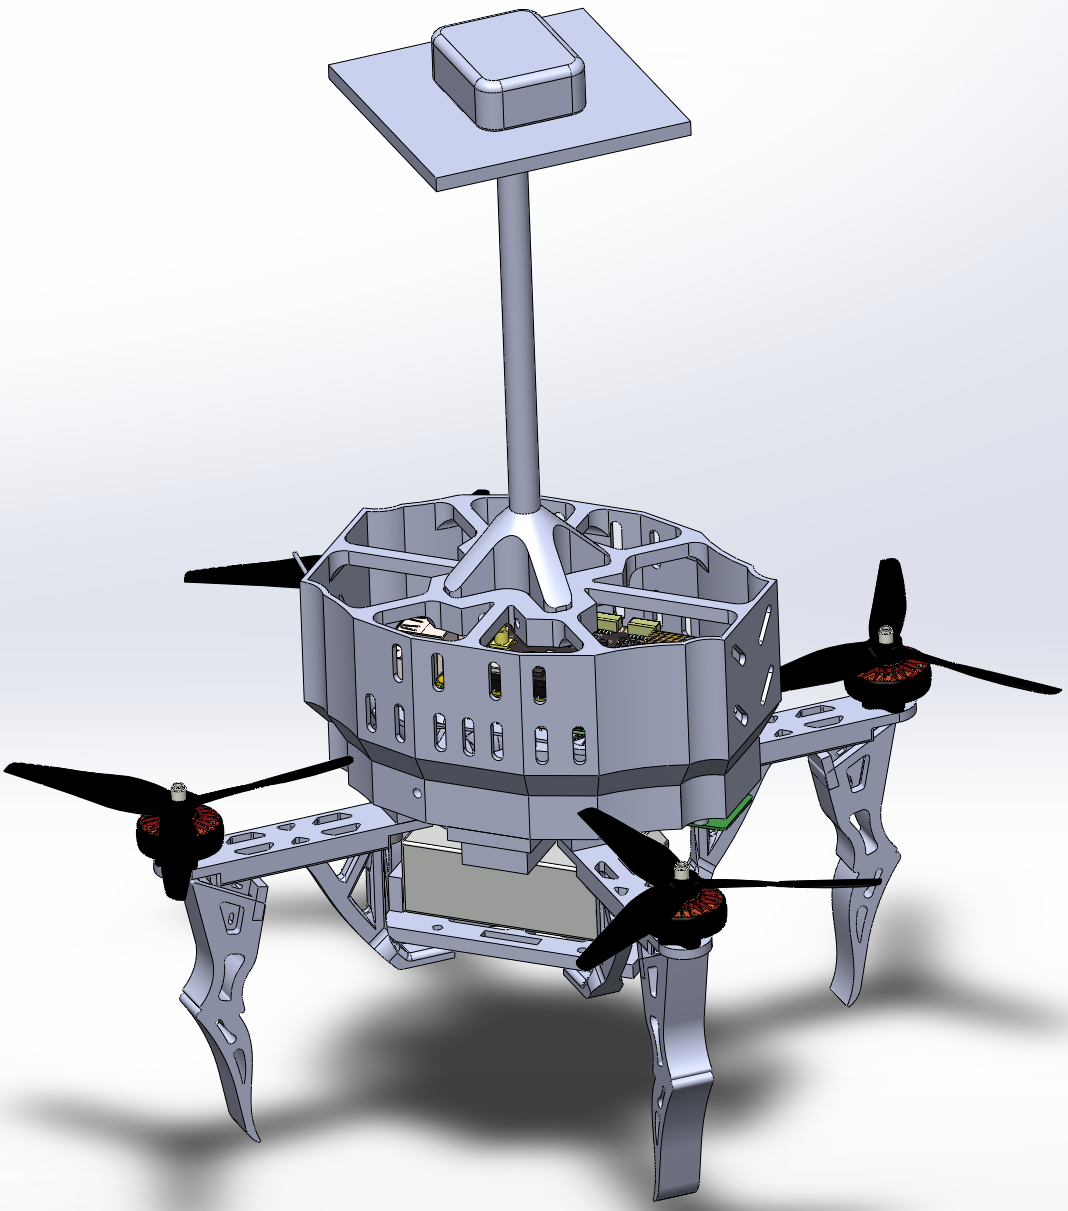
\includegraphics[width=0.9\textwidth]{CAD_Overview.png}
  \end{center}
\end{figure}

\clearpage

The overall component specifications are chosen in accordance to generally accepted specifications provided by \href{https://oscarliang.com/table-prop-motor-lipo-weight/}{Oscar Liang}, and are as follows:

\begin{table}[!h]
\begin{center}
\caption {General Design Specifications}
\label{tab:genDesignSpecs}
\begin{tabular}{ | m{7cm} | m{8cm} | } 
\hline
Frame Size & 210mm \\
\hline
Prop Size & 5 inch \\
\hline
LiPo Battery & 1000 - 1300mAh 3s/4s \\
\hline
Motor KV & 2300KV - 2700KV \\
\hline
Motor Stator Size & 2204 - 2206 \\
\hline
Weight without Battery & 250g - 450g \\
\hline
\end{tabular}
\end{center}
\end{table}

The components are then attached through M3 button head hex bolts and nuts to maintain a low bolt profile and weight.
Particular consideration is also given to minimizing the vibrations and Electromagnetic (EM) interference that the sensors on the Navio2 are subjected to.

Each component is defined in further detail within \nameref{tab:MechHardware} with the CAD shown within \nameref{sec:mechHardwareAppendix}.

\begin{landscape}
\begin{table}[!h]
\begin{center}
\caption {Mechanical Hardware Components}
\label{tab:MechHardware}
\begin{tabular}{ | m{2.7cm} | m{1.9cm} | m{1.4cm} | m{5.5cm} | m{10.3cm} | } 
\hline
Component & Acquisition & Material & Fabrication Method & Design Explanation \\
\hline
\nameref{Battery Compartment} & Built & PLA & 3D printed from CAD. 0.2mm layer height, 2 layer perimeter, 50\% gyroid infill. & 
    Separate compartment created below drone to isolate and protect battery against other components, and maintain a central center of balance. Battery also kept farthest away from Navio2 to minimize EM interference to sensors. \\
\hline
\nameref{Frame Arm} (x4) & Built & PLA & 3D printed from CAD. 0.2mm layer height, 4 layer perimeter, 50\% gyroid infill. & 
    Removable arms to facilitate repairs upon damage or design changes. \\
\hline
\nameref{Landing Leg} (x4) & Built & PLA & 3D printed from CAD. 0.2mm layer height, 4 layer perimeter, 50\% gyroid infill. & 
    Removable landing legs to facilitate repairs, and prevent damage to the drone's lower frame upon landing. \\
\hline
\nameref{GPS Mast} & Built & PLA & 3D printed from CAD. 0.2mm layer height, 12 layer perimeter, 20\% gyroid infill. Top part covered with foil tape to provide metallic plane. & 
    To elevate the GPS 20cm above the electrical components and provide a metallic plane to boost GPS signals. Mast also mounted close to center of drone to maintain a central center of balance. \\
\hline
\nameref{Enclosure} & Built & PLA & 3D printed from CAD. 0.3mm layer height, 4 layer perimeter, 20\% gyroid infill. & 
    Enclosure for electrical components and wiring. Prevents damage from the propellors, external forces, and the environment. Cutout slots available on sides to reduce weight and allow anchor points for zip ties of wiring. \\
\hline
\nameref{Top Plate} & Built & PLA & 3D printed from CAD. 0.2mm layer height, 2 layer perimeter, 50\% gyroid infill. & 
    Main mounting plate for electronic components. Features slots and holes to attach electrical components. Attaches to a dampening plate that holds the Raspberry Pi and Navio2. X-Frame design chosen for simplicity in design and ease of control. \\
\hline
\nameref{Dampening Plate} & Built & PLA & 3D printed from CAD. 0.2mm layer height, 2 layer perimeter, 50\% gyroid infill. & 
    Dampening plate to mount the Raspberry Pi and Navio2. Attaches to the Top Plate through four dampening balls, and minimizes vibrations to the Raspberry Pi and Navio2. \\
\hline
Dampening Balls (x4) & Bought & Silicone Rubber & -- & 
    Dampening balls to absorb vibrations from the frame. \\
\hline
\nameref{Propeller} (x4) & Bought & PC & -- & 
    5.1 inch diameter, 3.4 inch pitch, triblade design. \\
\hline
Aluminum Foil Tape & Bought & Aluminum & -- & 
    To provide a metallic ground plane for the GPS, and to provide EM protection on battery power wires. \\
\hline
\end{tabular}
\end{center}
\end{table}
\end{landscape}

\clearpage

\section{Design of Electrical Components}
\label{sec:elecComponents}

The major electrical components are selected in accordance to Table \ref{tab:genDesignSpecs}, with the use of the Navio2 as the premade flight controller. The decision to use the Navio2 as opposed to creating a flight controller from scratch is further explored within \nameref{sec:Reflection}. The Raspberry Pi 3B is then used to run the image processing and control logic of the drone. The overall schematic of the drone is shown in Figure \ref{elecSchematic}, with the individual components defined in Table \ref{tab:elecComponents}.

\begin{figure}[h!]
  \begin{center} 
  \caption{Electrical Schematic}
  \label{elecSchematic}
        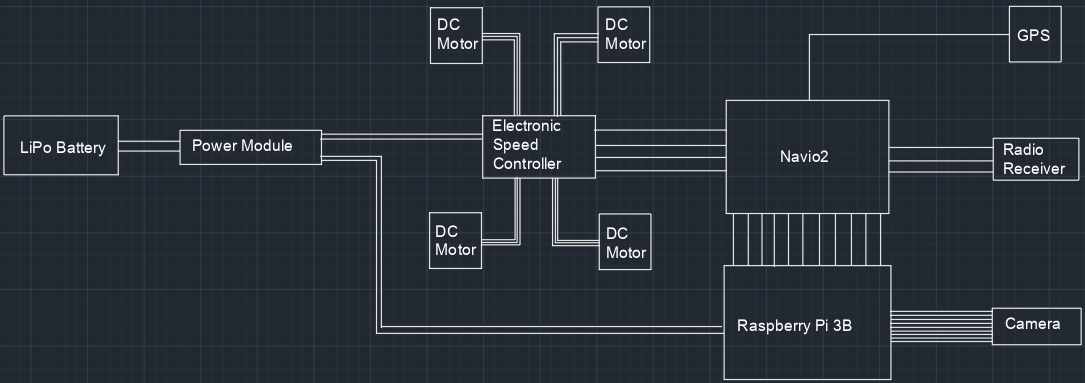
\includegraphics[width=1\textwidth]{ElectricalSchematic.PNG}
  \end{center}
\end{figure}

\begin{table}[!h]
\begin{center}
\caption {Electrical Components}
\label{tab:elecComponents}
\begin{tabular}{ | m{2.7cm} | m{1.9cm} | m{4cm} | m{6.4cm} | } 
\hline
Component & Acquisition & Specifications & Design Explanation \\
\hline
\nameref{Raspberry Pi 3B} & Bought & 1.2GHz Broadcom CPU, 1GB RAM, 40 Pin GPIO & 
    Main controller for drone. Responsible for running software components. \\
\hline
\nameref{Navio2} & Bought & Redundant power supply with built in barometer, accelerometer, gyro, and compass. & 
    Hat for Raspberry Pi, providing all the required sensors for operation. Also supported by Ardupilot software and runs interfaces with Debian, a real time Linux OS. \\
\hline
\nameref{Radio Antenna and Receiver} & Bought & 2.4GHz Frequency & 
    Redundant communication method and for development/testing. Will not be used by the operator. \\
\hline
\nameref{Camera} & Bought & 5MP 1080p Camera & 
    To acquire visual data. Infrared cameras not required due to operation of drone only during daytime periods or under well lit parking lot. \\
\hline
\nameref{Electronic Speed Controller} & Bought & 4 in 1 45A ESC & 
    To control the motors given PWM signals from the Navio2. \\
\hline
\nameref{GPS} & Bought & U-Blox NEO-M8N & 
    To acquire localization of the drone. \\
\hline
\nameref{Brushless DC Motor} (x4) & Bought & iFlight Xing 2205 2300kV. For full specs, see \nameref{motorSpecs}. & 
    To spin the propellors. \\
\hline
\nameref{LiPo Battery} & Bought & 1500mAh 4S 120C LiPo Battery & 
    To provide power to the drone. \\
\hline
\end{tabular}
\end{center}
\end{table}

\clearpage

\section{Design of Communication Protocols}
\label{sec:commProtocols}

Communication is required between the different modules of the product, as well as to the Operator. These communication protocols are defined in Table \ref{tab:commProtocols}.

\begin{table}[!h]
\begin{center}
\caption {Communication Protocols}
\label{tab:commProtocols}
\begin{tabular}{ | m{2.7cm} | m{4.5cm} | m{7.8cm} | } 
\hline
Component & Communication Between & Design Explanation \\
\hline
ROS Nodes & Interprocess communication on drone. &
    ROS allows the creation of a distribution of nodes, which communicate with one another through messages, called topics. The nodes can either subscribe or publish topics without any dependency on other nodes. Thus, each module can be developed as an independent node, allowing for encapsulation of each module. \\
\hline
MavROS & Ardupilot, the flight controller, and the Drone Software. &
    MavROS is a package within ROS that allows for reading and publishing MAVLink messages, which originate from Ardupilot. These messages contain the raw sensor data and other data provided by the flight controller. From the published topics from MavROS, other nodes within the Drone Software will then read the topics. Services are also offered by MavROS, allowing for sending commands to Ardupilot. \\
\hline
Local Area Network (LAN) Wifi & Drone Software and Operator's Application. &
    A LAN is created through a USB router connected to the Operator's PC. Both the Operator's PC and the drone shall connect to this LAN, allowing for communication between the devices though network sockets. Communication will be handled within the DroneSocket and OperatorSocket modules, and supports the usage of synchronous and asynchronous messages. \\
\hline
Graphical User Interface (GUI) & Operator's Application and Operator. &
    A GUI is used as the Human Machine Interface (HMI) due to the lower technical skill required, and to reduce training times required to operate the product. \\
\hline
\end{tabular}
\end{center}
\end{table}

\clearpage

\section{Timeline}
\label{sec:timeline}

Individual timelines are provided to each major component of the product, and are defined within \nameref{tab:mechTimeline}, \nameref{tab:elecTimeline}, \nameref{tab:commTimeline}, and \nameref{tab:moduleTimeline}. The modules mentioned within \nameref{tab:moduleTimeline} are defined in further detail within the  \href{https://github.com/icecap360/DroneCapstone/blob/master/docs/Design/SoftDetailedDes/MIS.pdf}{Module Interface Specifications} document.

\begin{table}[!h]
\begin{center}
\caption {Mechanical Hardware Timeline}
\label{tab:mechTimeline}
\begin{tabular}{ | m{2.5cm} | m{7.5cm} | m{3cm} | m{2cm} | } 
\hline
Date & Components/Description & Test Method & Responsible By \\
\hline
October 10, 2022 & Place order for all bought components. Includes dampening balls and propellers. & 
    -- & Ali, Fady, Winnie, Zaid \\
\hline
November 8, 2022 & Design, fabricate, and test mounting plates and basic structure of the drone. Includes the Battery Compartment, Frame Arm, Top Plate, and Dampening Plate. & 
    Test mounting of all electronic components. & Winnie \\
\hline
December 12, 2022 & Design, fabricate, and test Landing Legs and mounts for external sensors such as the camera and GPS. & 
    Test mounting of camera and GPS. & Winnie \\
\hline
December 14, 2022 & All components. & 
    Test flight. & Ali, Fady, Winnie, Zaid \\
\hline
January 9, 2023 & Implement improvements to design from previous test flight. Includes the design and fabrication of the Enclosure, and revisions to other parts to improve structural integrity. & 
    Reassemble drone with new components. & Winnie \\
\hline
January 23, 2023 & All components. & 
    Test flight. & Ali, Fady, Winnie, Zaid \\
\hline
January 30, 2023 & Revise design if required from previous test flight. & 
    Reassemble drone with new components. & Winnie \\
\hline
\end{tabular}
\end{center}
\end{table}

\begin{table}[!h]
\begin{center}
\caption {Electrical Components Timeline}
\label{tab:elecTimeline}
\begin{tabular}{ | m{2.5cm} | m{7.5cm} | m{3cm} | m{2cm} | } 
\hline
Date & Components/Description & Test Method & Responsible By \\
\hline
October 10, 2022 & Place order for all bought components. Includes all electronic components. & 
    -- & Ali, Fady, Winnie, Zaid \\
\hline
October 24, 2022 & Raspberry Pi and Navio2. & 
    Verify sensor readings and communication with Raspberry Pi. & Ali, Fady \\
\hline
November 14, 2022 & Connect battery, ESC, and motors to Raspberry Pi. & 
    Test motor movement and perform ESC calibration. & Fady \\
\hline
December 14, 2022 & All components. & 
    Test flight. & Ali, Fady, Winnie, Zaid \\
\hline
January 9, 2023 & Reassemble wiring to create more secure connections. & 
    Verify motor movement and sensor readings. & Fady \\
\hline
January 23, 2023 & All components. & 
    Test flight. & Ali, Fady, Winnie, Zaid \\
\hline
January 30, 2023 & Revise electrical design if required from previous test flight. & 
    Verify motor movement and sensor readings. & Fady \\
\hline
\end{tabular}
\end{center}
\end{table}

\begin{table}[!h]
\begin{center}
\caption {Communication Protocols Timeline}
\label{tab:commTimeline}
\begin{tabular}{ | m{1.7cm} | m{6.7cm} | m{4.6cm} | m{2cm} | } 
\hline
Date & Components/Description & Test Method & Responsible By \\
\hline
October 13, 2022 & Establish LAN communication between PC and drone. & 
    SSH into Raspberry Pi and verify bidirectional communication. & Ali, Winnie \\
\hline
October 17, 2022 & Establish MavROS communication with the flight controller. & 
    Verify sensor readings sent by the flight controller, and ability to send commands to the flight controller. & Ali, Fady, Winnie \\
\hline
December 5, 2022 & Establish LAN communication between Windows PC and Software in the Loop (SITL) testing environment. The SITL testing environment is a series of applications that run on a Linux virtual machine. & 
    Demonstrate that a sample message (like 'Hello World') between separate python applications running on the two environments. & Zaid \\
\hline
December 25, 2022 & Write modules that present a usable interface for other modules to easily send and receive data. 
    Create modules to simplify the usage of ROS services and topics offered by MavROS and for sending and receiving JSON messages between the python applications running on the drone and PC. Given that the SITL environment replicates the drone environment, communication modules designed for the drone will also work on the SITL environment. & 
    Unit test the communication modules. For example, print the accelerometer values to the screen. Send and receive sample messages (like 'Hello World'). & Zaid \\
\hline
December 28, 2022 & Establish the ability to read live camera images, annotate the images, and send live image from the drone's camera to the Windows PC. & 
    Watch live camera output seen on the Windows PC. Also annotate some text, such as 'Hello World' in the bottom left hand corner to verify that the image annotation works. & Ali \\
\hline
December 29, 2022 & Create a simple to use module that gets live images from the camera, send images to the operator's PC, and receive images to the operator's PC. & 
    Unit test the modules by watching live camera output on the Windows PC. & Ali \\
\hline
\end{tabular}
\end{center}
\end{table}

\begin{table}[!h]
\begin{center}
\caption {Modules Timeline}
\label{tab:moduleTimeline}
\begin{tabular}{ | m{2.5cm} | m{7.5cm} | m{3cm} | m{2cm} | } 
\hline
Date & Modules/Description & Test Method & Responsible By \\
\hline
December 25, 2022 & DroneSocket, OperatorSocket & 
    Unit test the communication modules. For example, print the accelerometer values to the screen. Send and receive sample messages (like 'Hello World'). & Ali \\
\hline
December 25, 2022 & DroneSocket, OperatorSocket & 
    Unit test the communication modules. For example, print the accelerometer values to the screen. Send and receive sample messages (like 'Hello World'). & Ali \\
\hline
\end{tabular}
\end{center}
\end{table}

[todo]

\clearpage

% \bibliographystyle {plainnat}
% \bibliography{../../../refs/References}

\newpage{}

\appendix

\section{Mechanical Hardware}
\label{sec:mechHardwareAppendix}

\begin{figure}[h!]
  \begin{center} 
  \caption{Exploded CAD}
  \label{ExplodedCAD}
        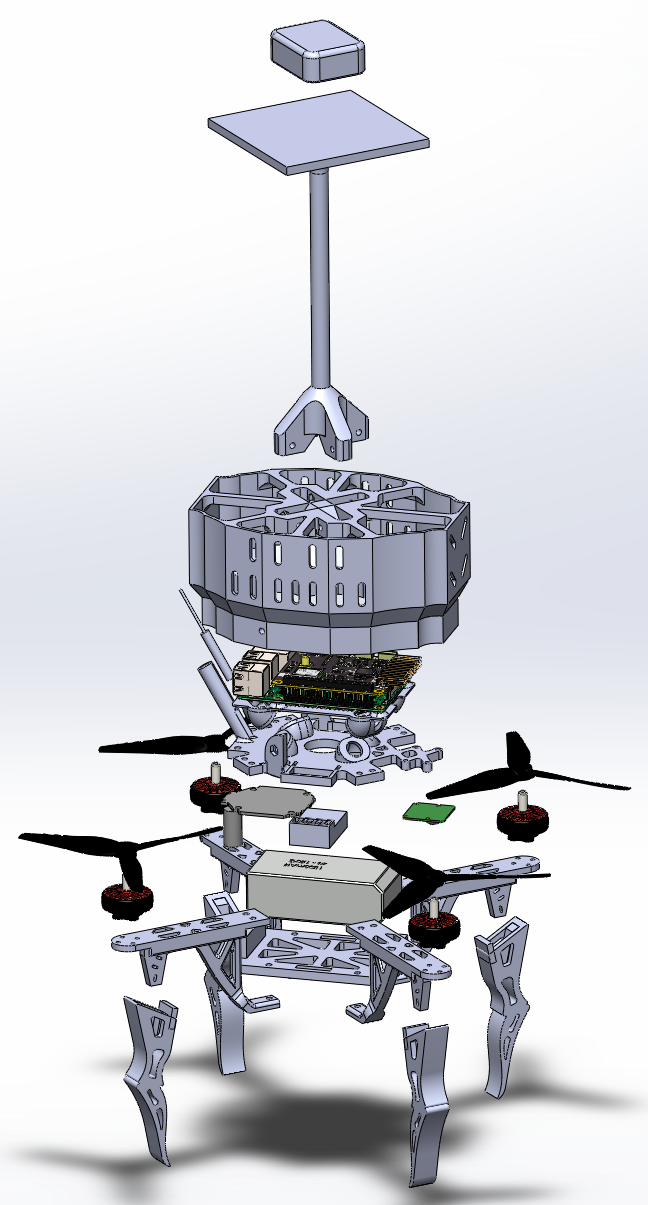
\includegraphics[width=0.65\textwidth]{CAD_Exploded.png}
  \end{center}
\end{figure}

\begin{figure}[h!]
  \begin{center} 
  \caption{Battery Compartment}
  \label{Battery Compartment}
        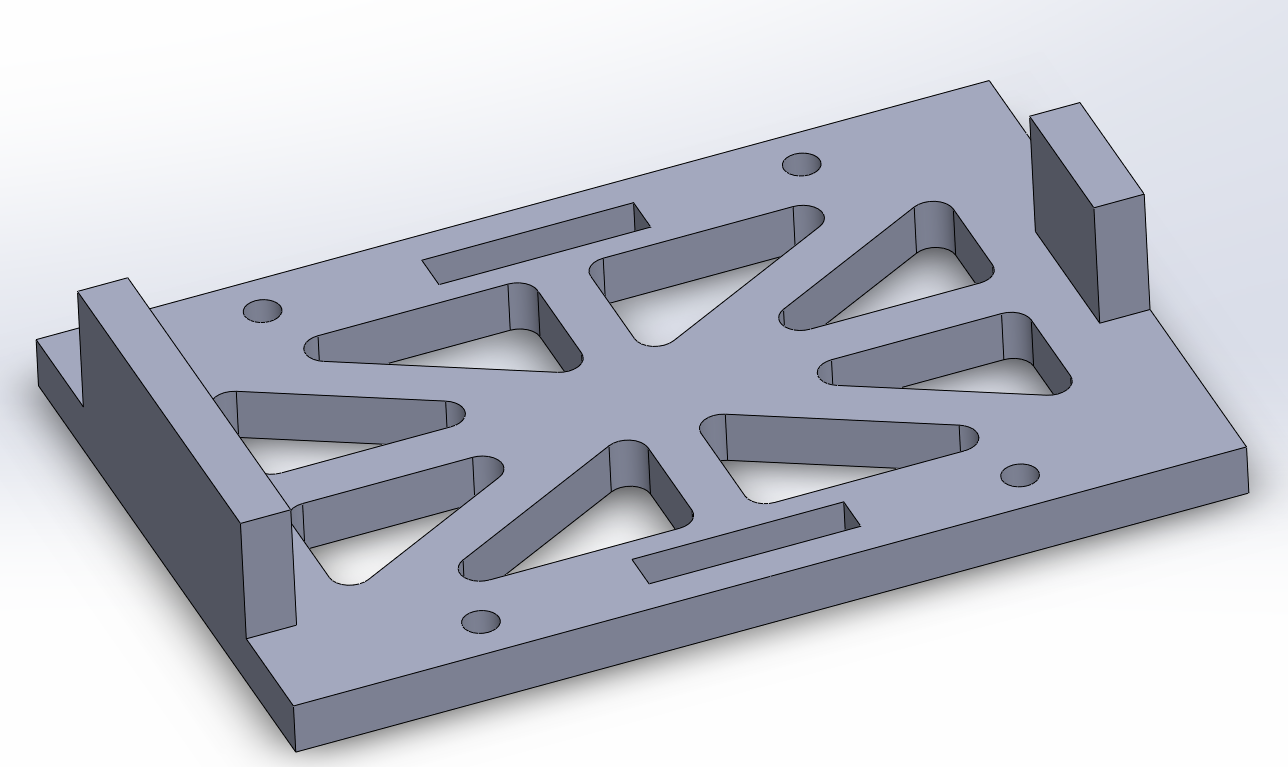
\includegraphics[width=0.65\textwidth]{CAD_BottomPlate.png}
  \end{center}
\end{figure}

\begin{figure}[h!]
  \begin{center} 
  \caption{Frame Arm}
  \label{Frame Arm}
        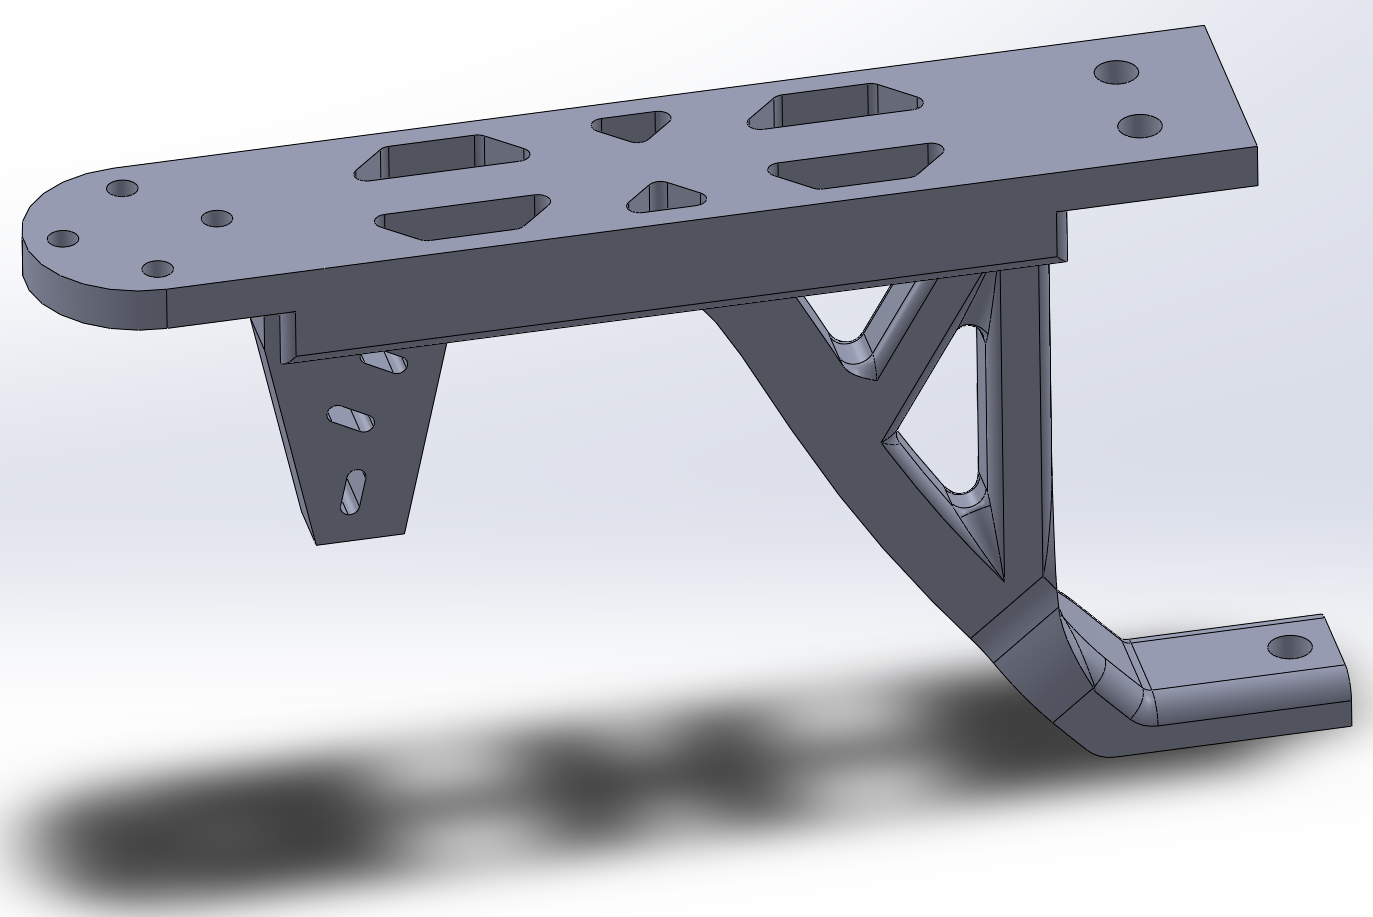
\includegraphics[width=0.65\textwidth]{CAD_Arm.png}
  \end{center}
\end{figure}

\begin{figure}[h!]
  \begin{center} 
  \caption{Landing Leg}
  \label{Landing Leg}
        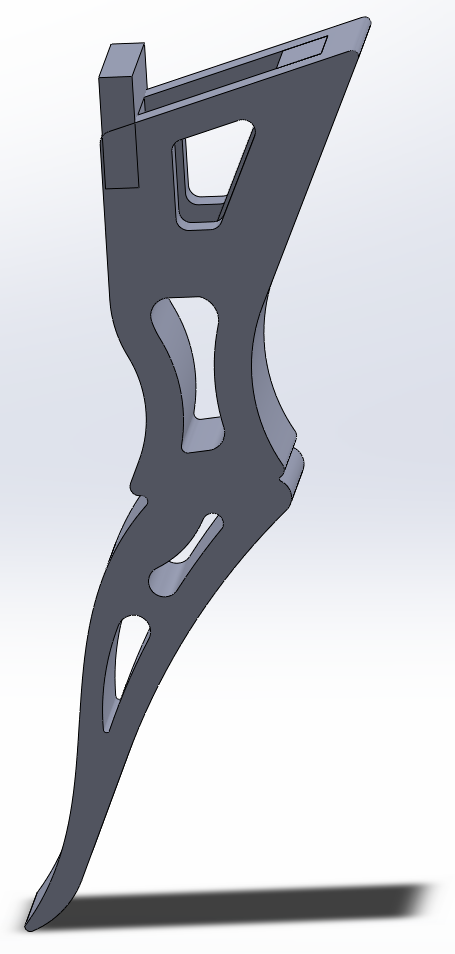
\includegraphics[width=0.35\textwidth]{CAD_Leg.png}
  \end{center}
\end{figure}

\begin{figure}[h!]
  \begin{center} 
  \caption{GPS Mast}
  \label{GPS Mast}
        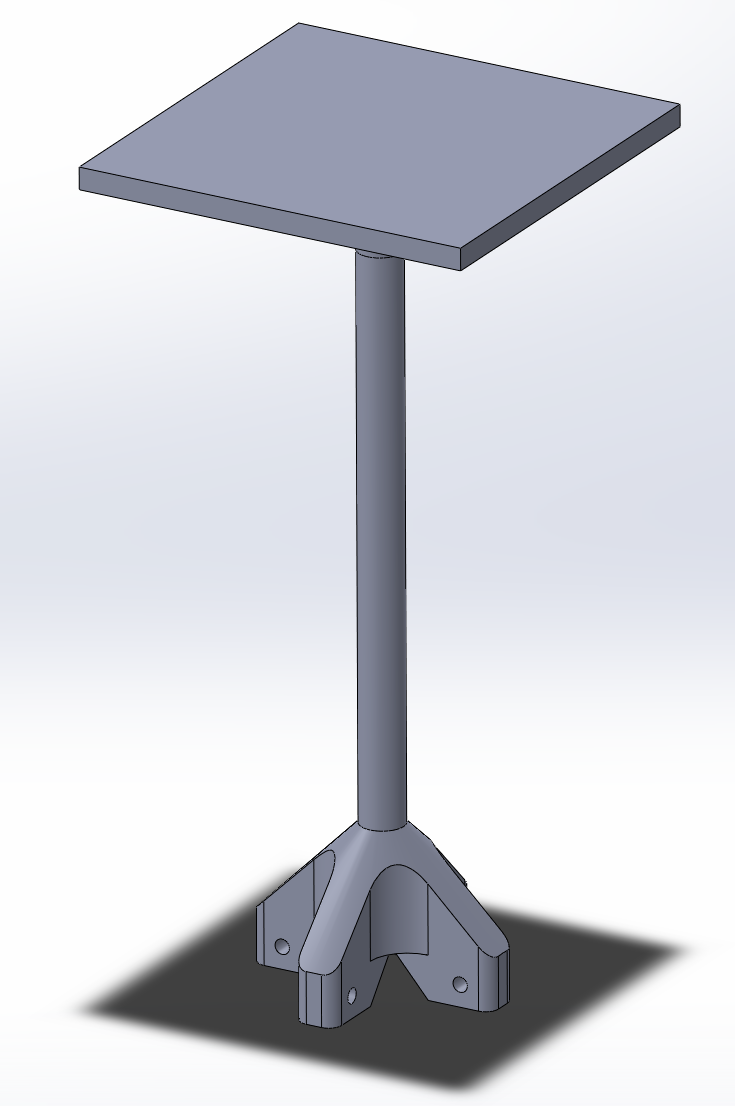
\includegraphics[width=0.45\textwidth]{CAD_Mast.png}
  \end{center}
\end{figure}

\begin{figure}[h!]
  \begin{center} 
  \caption{Enclosure}
  \label{Enclosure}
        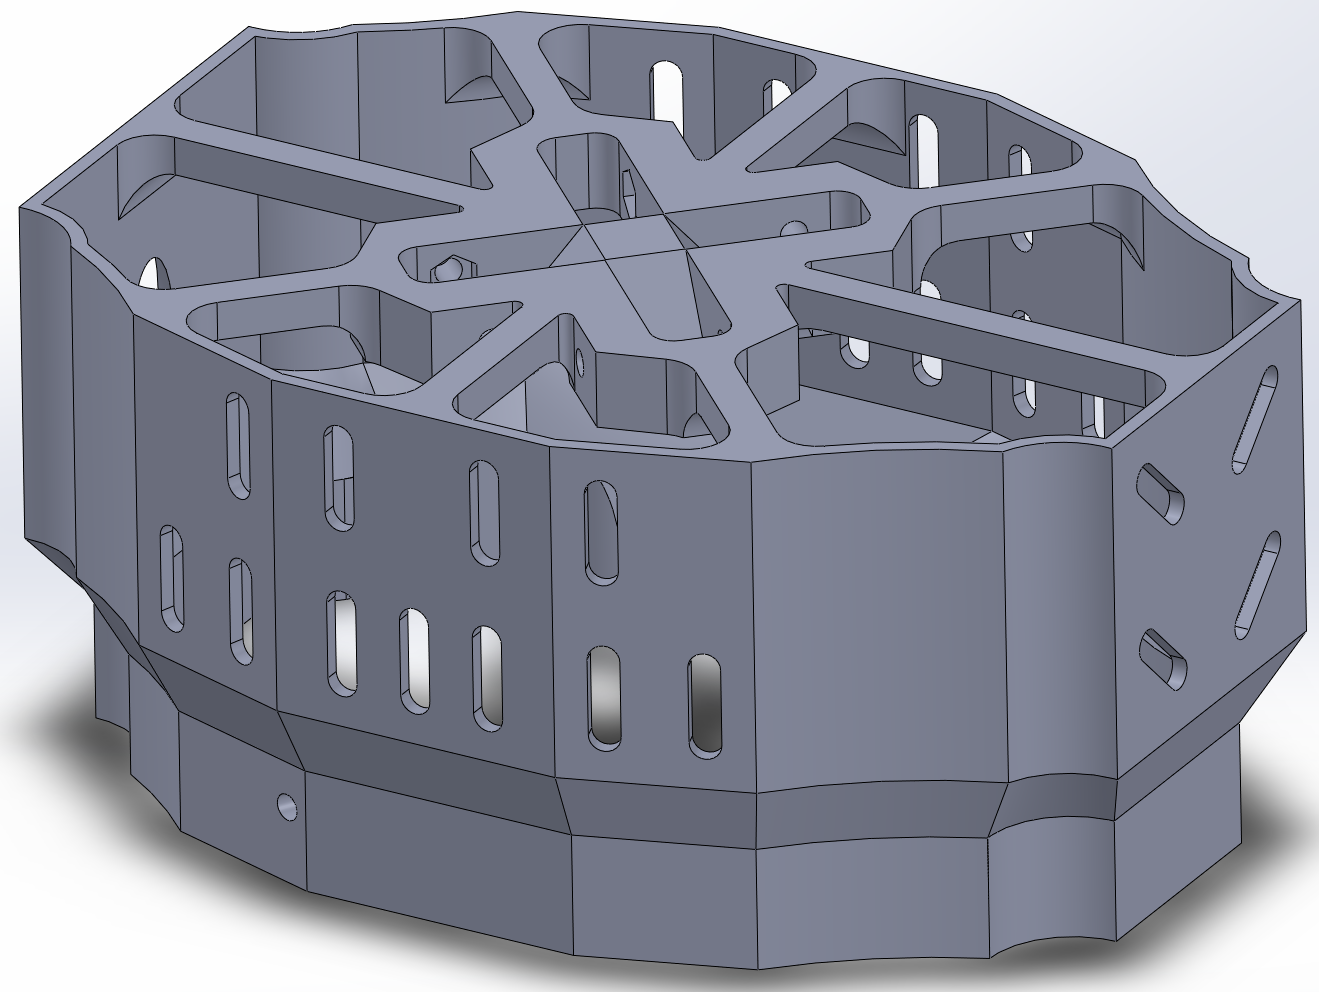
\includegraphics[width=0.65\textwidth]{CAD_Enclosure.png}
  \end{center}
\end{figure}

\begin{figure}[h!]
  \begin{center} 
  \caption{Top Plate}
  \label{Top Plate}
        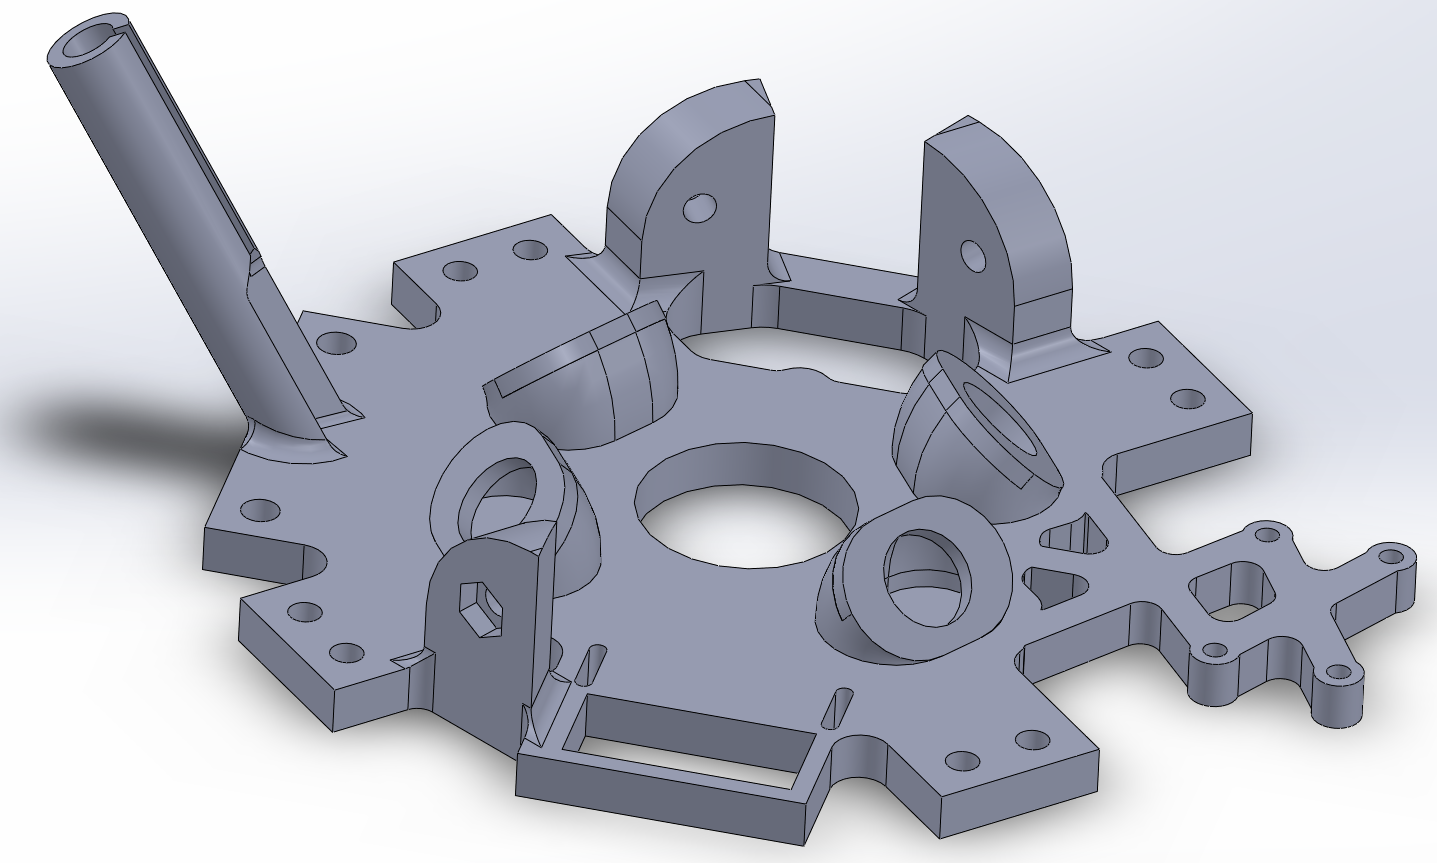
\includegraphics[width=0.65\textwidth]{CAD_TopPlate.png}
  \end{center}
\end{figure}

\begin{figure}[h!]
  \begin{center} 
  \caption{Dampening Plate}
  \label{Dampening Plate}
        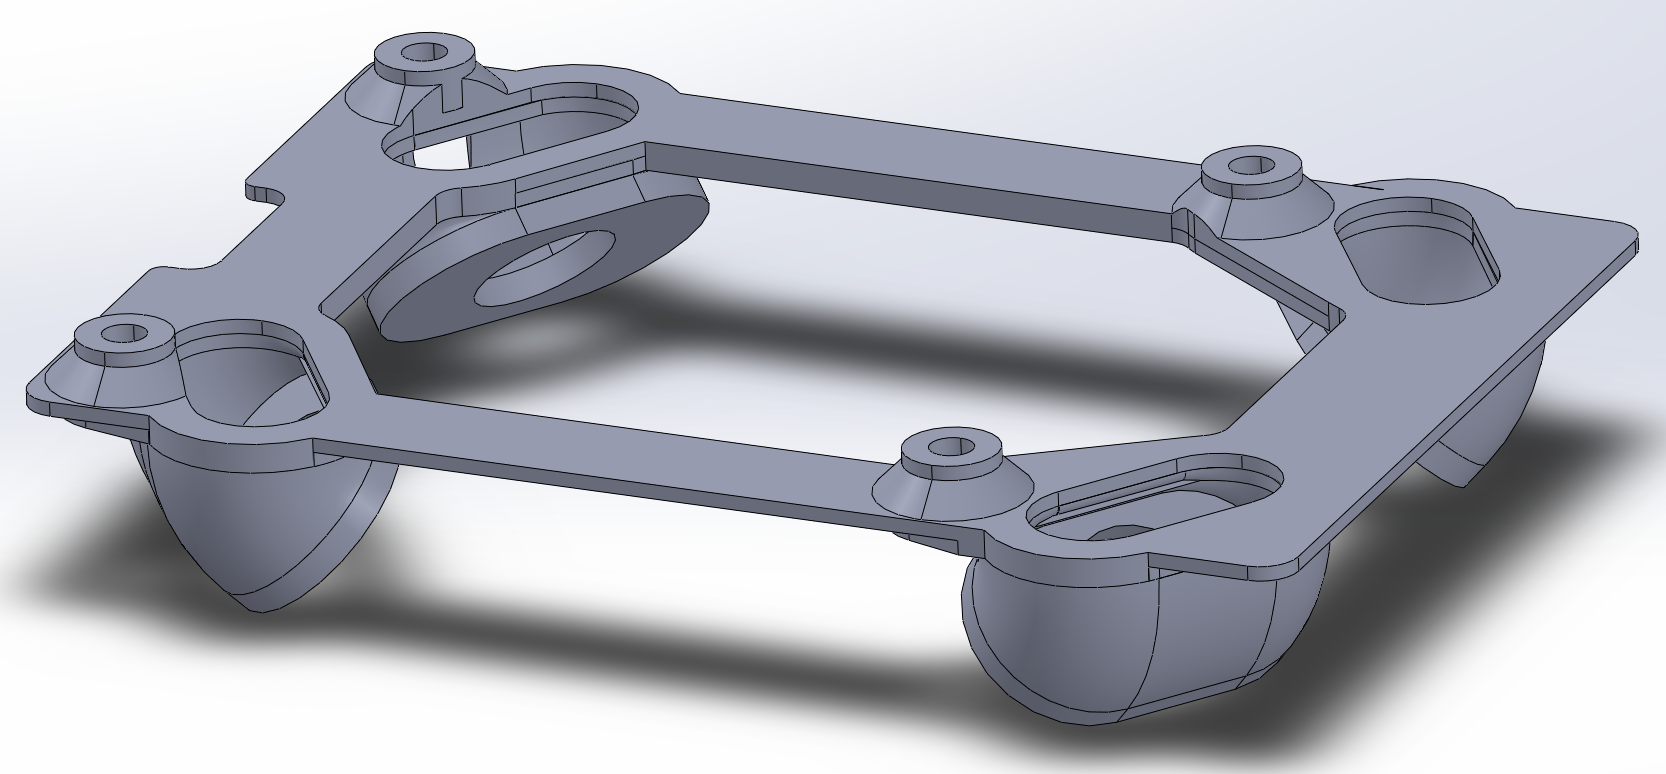
\includegraphics[width=0.65\textwidth]{CAD_DampenerTop.png}
  \end{center}
\end{figure}

\begin{figure}[h!]
  \begin{center} 
  \caption{Propeller}
  \label{Propeller}
        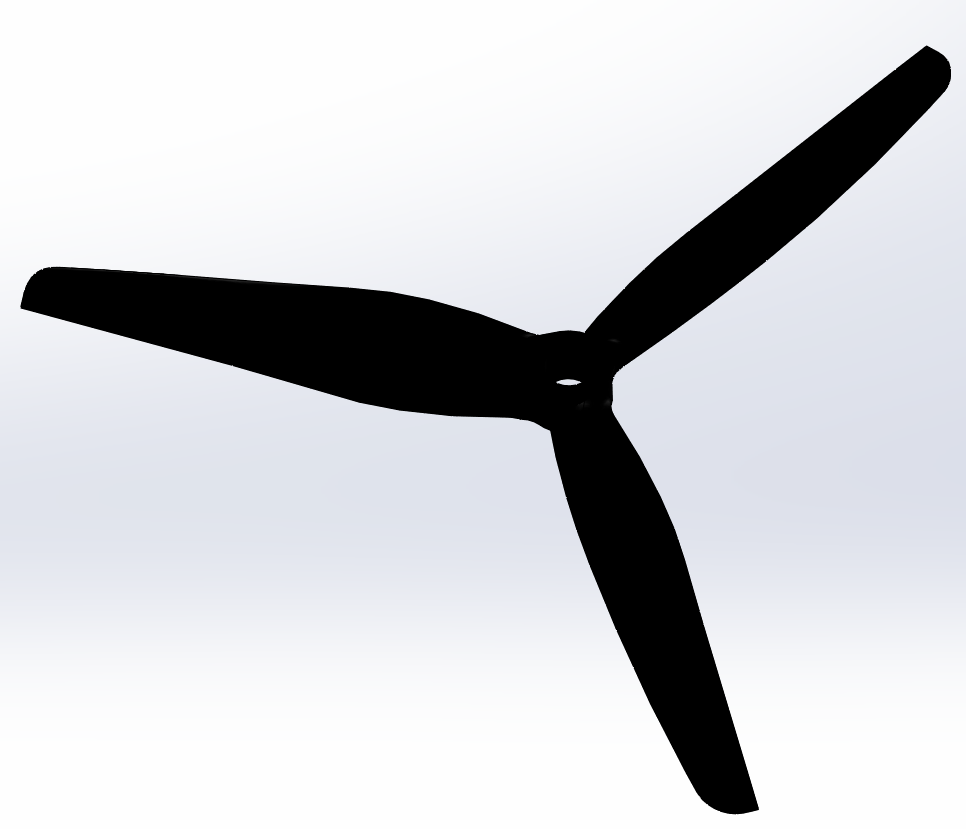
\includegraphics[width=0.65\textwidth]{CAD_Propeller.png}
  \end{center}
\end{figure}

\clearpage

\section{Electrical Components}

\begin{figure}[h!]
  \begin{center} 
  \caption{Raspberry Pi 3B}
  \label{Raspberry Pi 3B}
        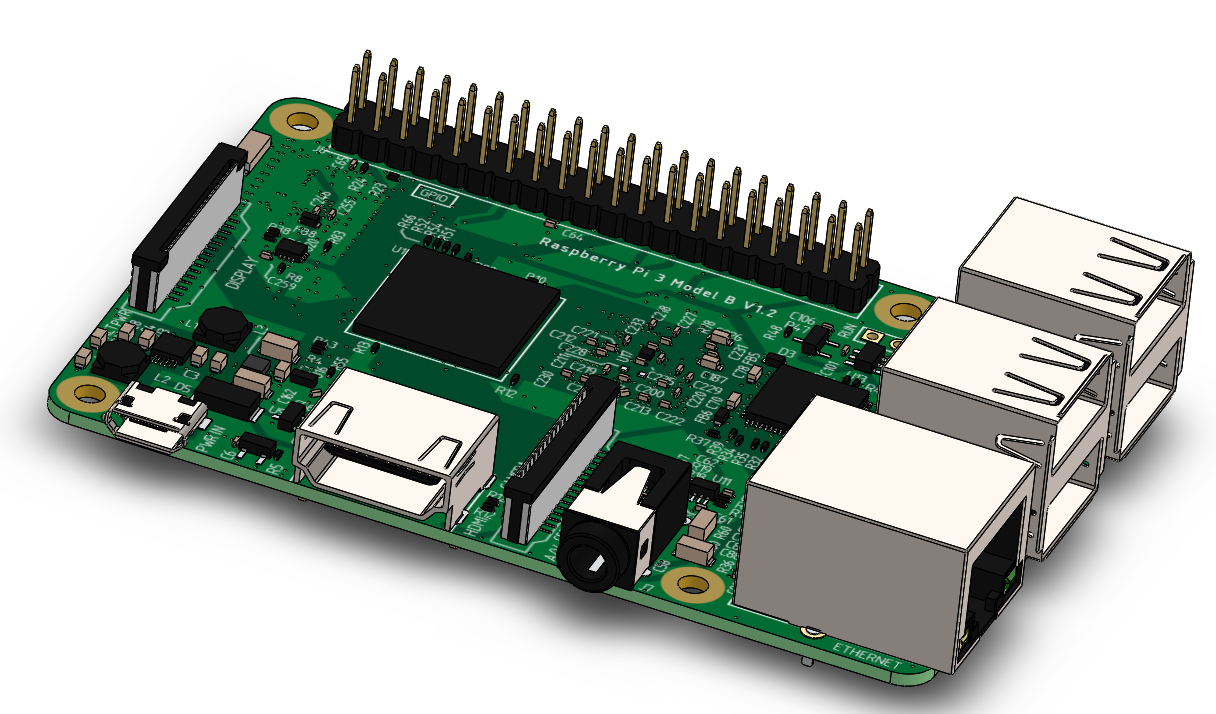
\includegraphics[width=0.65\textwidth]{CAD_RPi3B.png}
  \end{center}
\end{figure}

\begin{figure}[h!]
  \begin{center} 
  \caption{Navio2}
  \label{Navio2}
        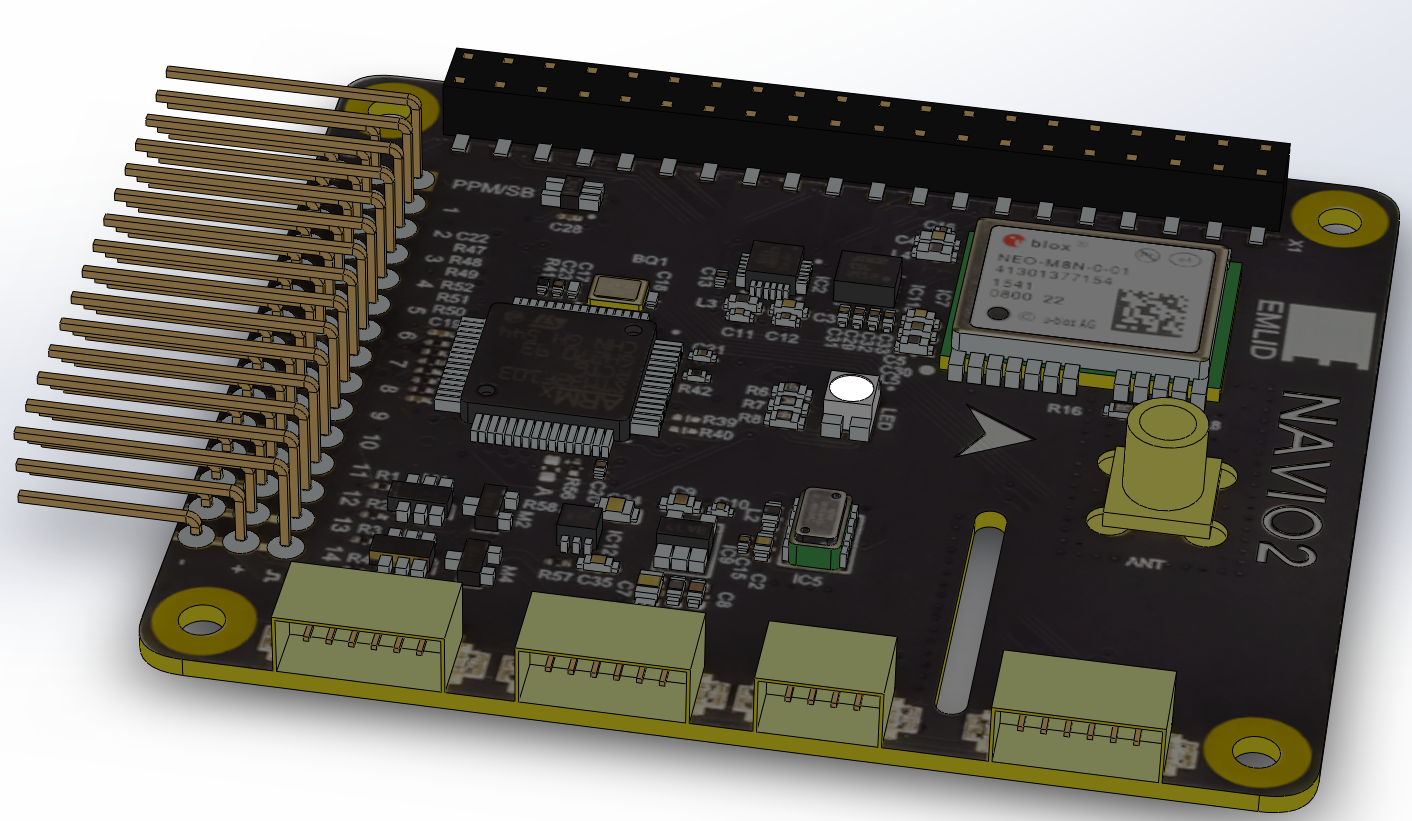
\includegraphics[width=0.65\textwidth]{CAD_Navio2.png}
  \end{center}
\end{figure}

\begin{figure}[h!]
  \begin{center} 
  \caption{Radio Antenna and Receiver}
  \label{Radio Antenna and Receiver}
        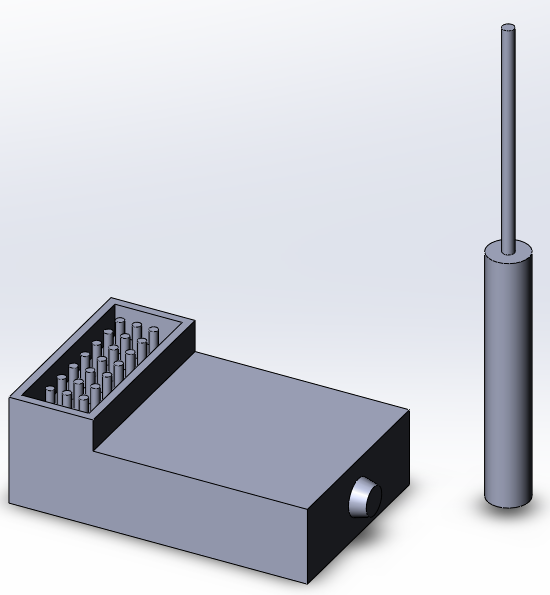
\includegraphics[width=0.45\textwidth]{CAD_Radio.png}
  \end{center}
\end{figure}

\begin{figure}[h!]
  \begin{center} 
  \caption{Camera}
  \label{Camera}
        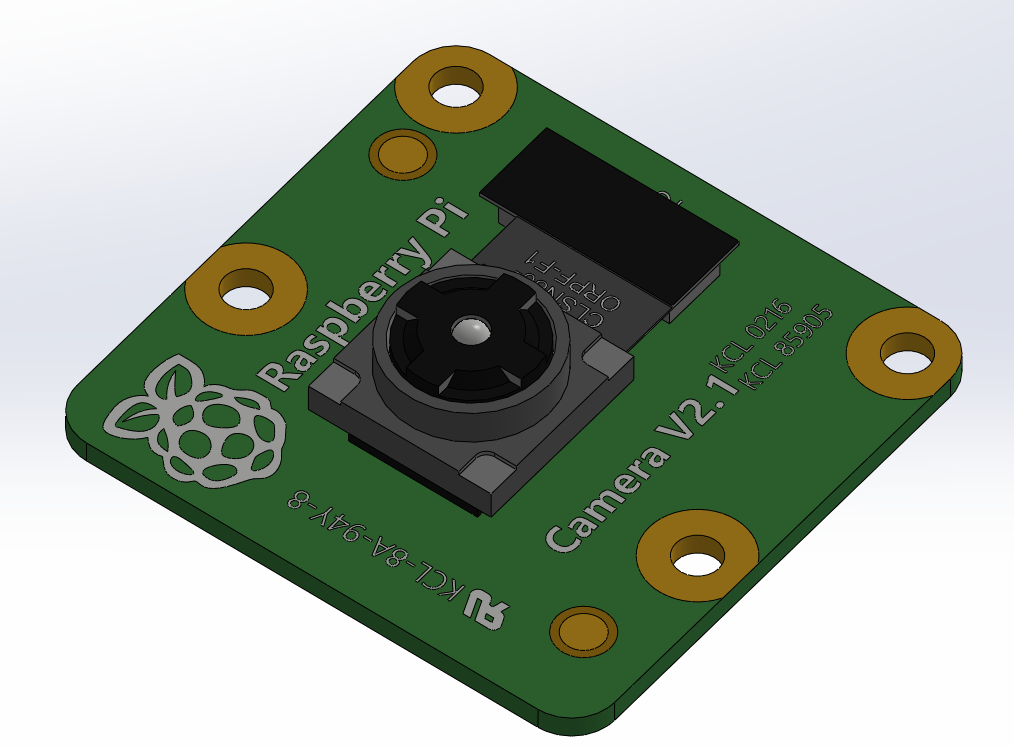
\includegraphics[width=0.65\textwidth]{CAD_Camera.png}
  \end{center}
\end{figure}

\begin{figure}[h!]
  \begin{center} 
  \caption{Electronic Speed Controller}
  \label{Electronic Speed Controller}
        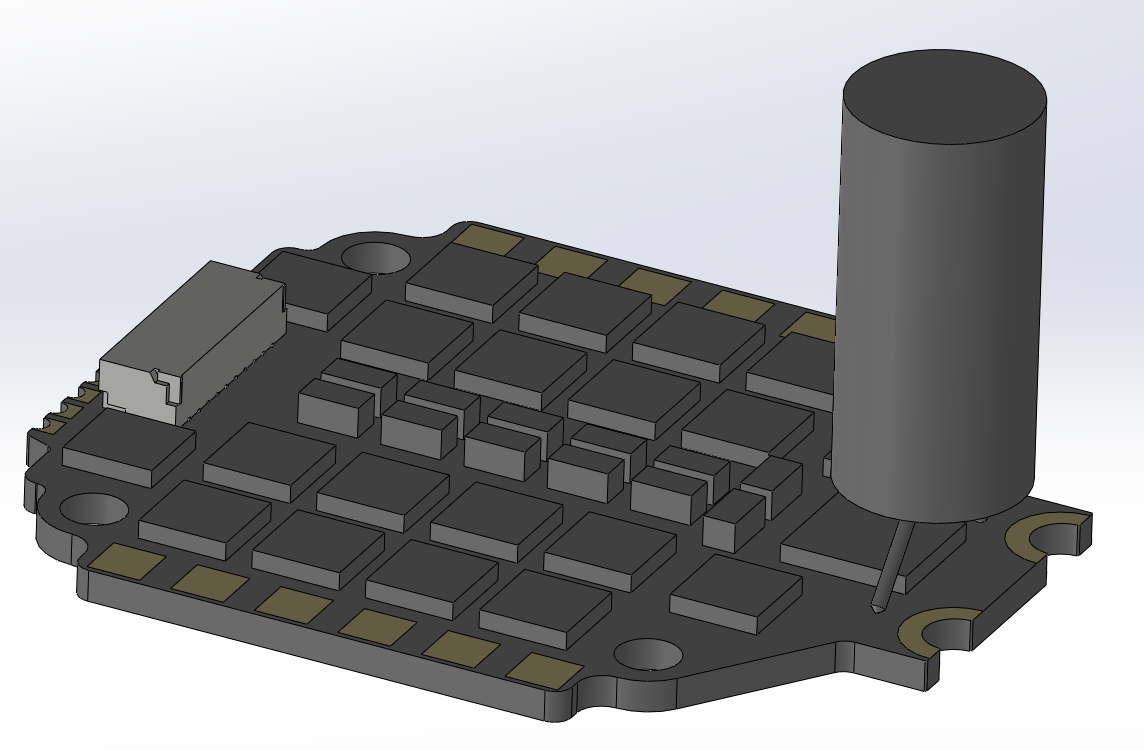
\includegraphics[width=0.65\textwidth]{CAD_ESC.png}
  \end{center}
\end{figure}

\begin{figure}[h!]
  \begin{center} 
  \caption{GPS}
  \label{GPS}
        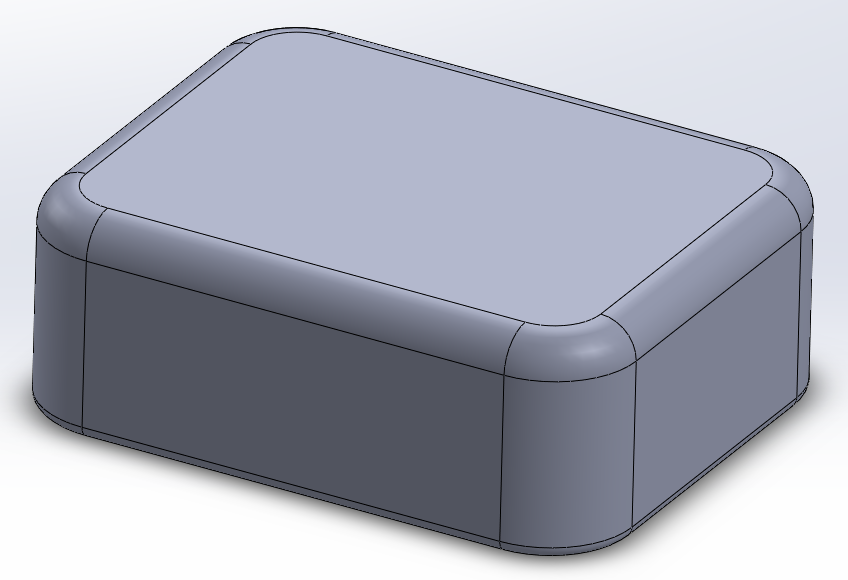
\includegraphics[width=0.45\textwidth]{CAD_GPS.png}
  \end{center}
\end{figure}

\begin{figure}[h!]
  \begin{center} 
  \caption{Brushless DC Motor}
  \label{Brushless DC Motor}
        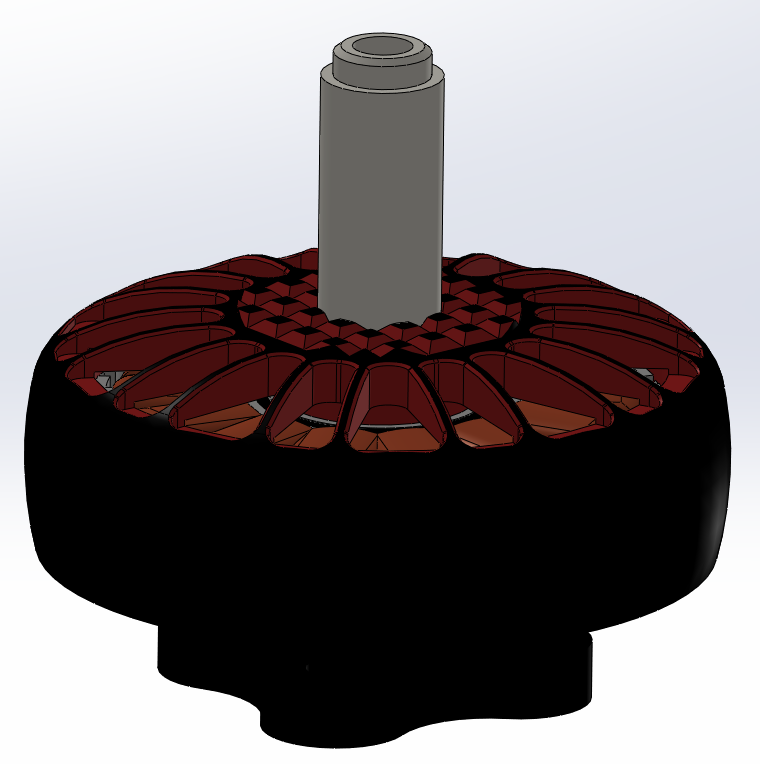
\includegraphics[width=0.45\textwidth]{CAD_Motor.png}
  \end{center}
\end{figure}

\begin{figure}[h!]
  \begin{center} 
  \caption{LiPo Battery}
  \label{LiPo Battery}
        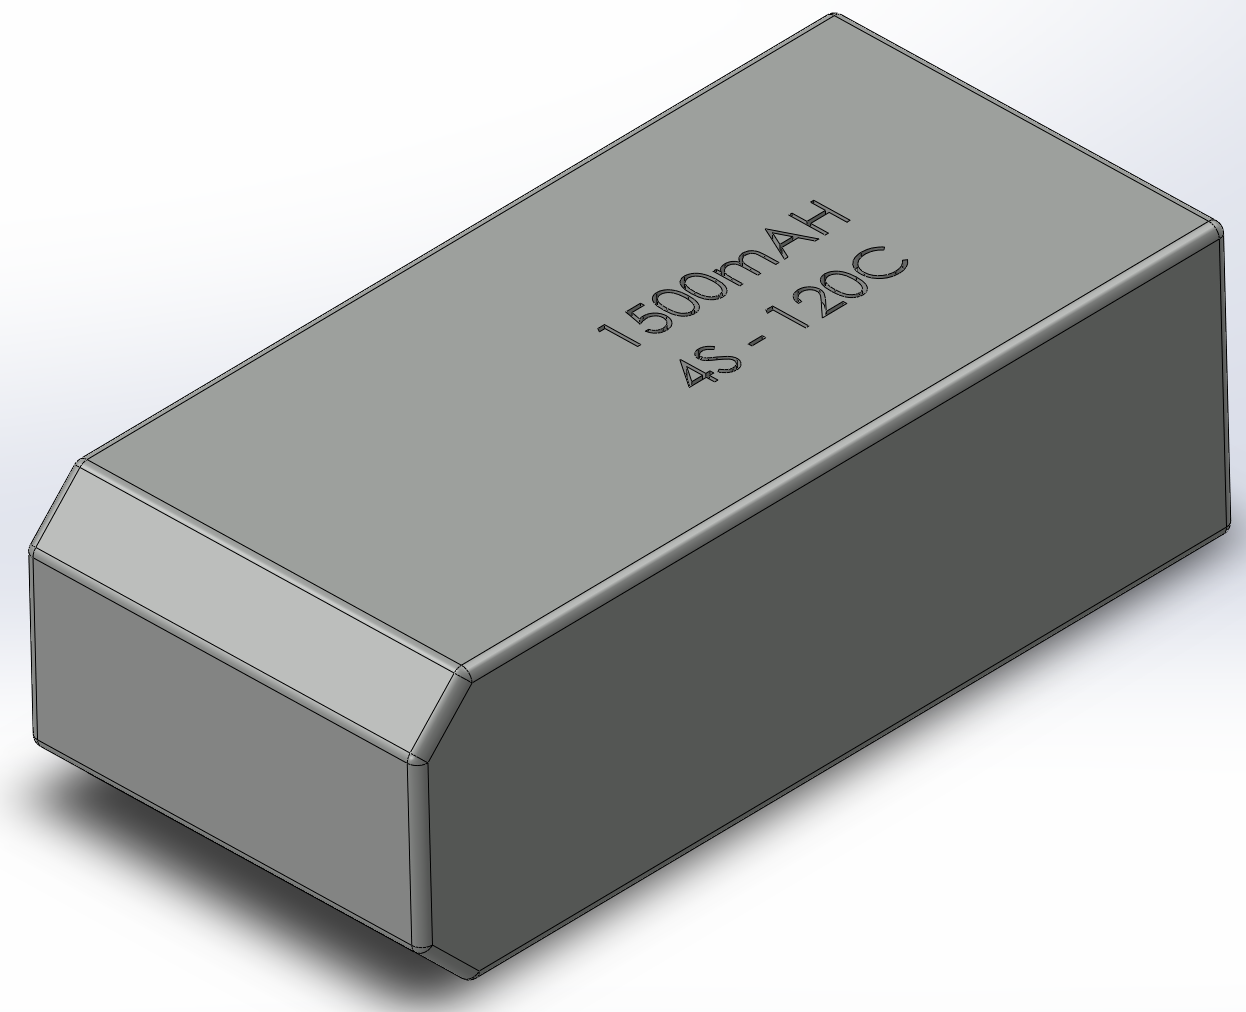
\includegraphics[width=0.45\textwidth]{CAD_Lipo.png}
  \end{center}
\end{figure}

\begin{figure}[h!]
  \begin{center} 
  \caption{Motor Specs}
  \label{motorSpecs}
        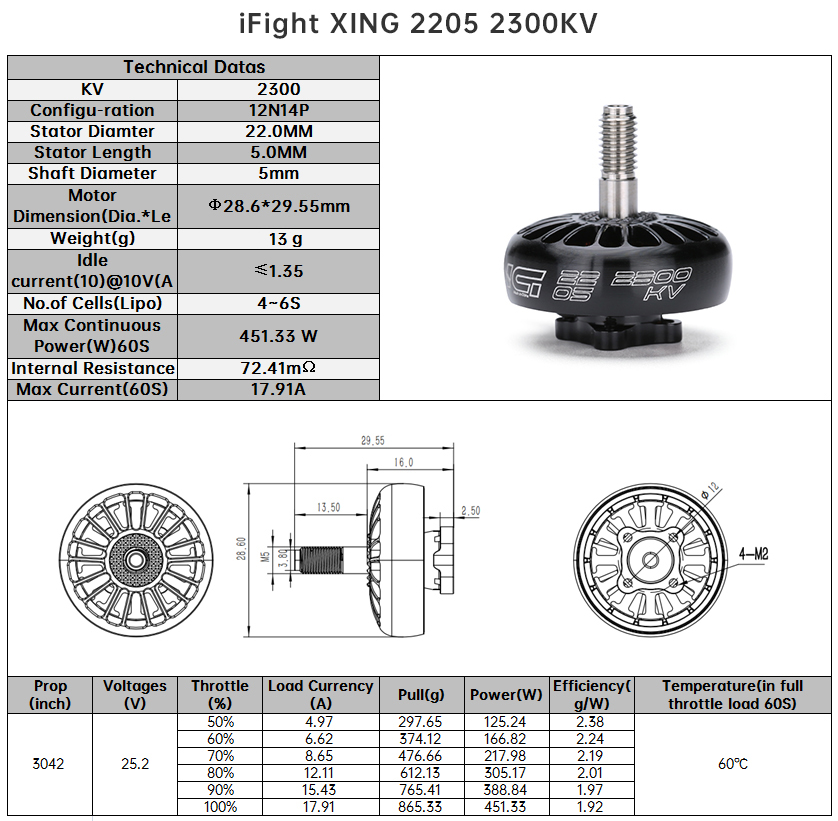
\includegraphics[width=0.65\textwidth]{iflightSpecs.png}
  \end{center}
\end{figure}

\clearpage

\section{Reflection}
\label{sec:Reflection}

Due to the limited resources available for the product, improvements to the product could be made if the resource constraint is removed. Such improvements are as follows:
\begin{enumerate}
    \item Improved camera dampeners to minimize vibrations on the camera during flight.
    \item Improved camera quality in terms of resolution and frames per second.
    \item Larger drone size and more powerful motors to allow for easier assembly, easier design, increased stability under inclement weather, and having room for for a secondary GPS, secondary camera, and additional sensors.
    \item Attach a wifi antenna onto the drone for increased connectivity range and switch camera communication to use a radio Video Transmitter (VTX) for increased bandwidth and speed.
    \item Larger battery capacity for increased flight times.
    \item More powerful edge compute device as compared to a Raspberry Pi 3B. Also requires switching the flight controller to a PixHawk instead of a Navio2, which is the industry standard for flight controllers and also provides support for additional edge compute devices.
    \item Substitute PLA for TPU for better vibration dampening qualities of the frame.
    \item Implement non-GPS localization for a redundant localization method, such as optical flow.
    \item Implement downward facing range finders, such as LiDAR or infrared, to give more accurate height readings and improve landing capabilities.
    \item Attach ultrasonic sensors in cardinal directions of the drone for object avoidance during flight.
\end{enumerate}

Multiple design solutions were also considered during the development of the ParkingLotHawk. The major alternatives are described within Table \ref{tab:designAlternatives}.

\begin{landscape}
\begin{table}[!h]
\begin{center}
\caption {Design Alternatives}
\label{tab:designAlternatives}
\begin{tabular}{ | m{4.5cm} | m{4.6cm} | m{6.5cm} | m{6.7cm} | } 
\hline
Design Alternative & Advantages & Disadvantages & Reason for Not Using Design Alternative \\
\hline
Create a land rover. & 
    \begin{enumerate}
        \item Longer battery life.
        \item Lower maintenance.
        \item Operable in more diverse environmental conditions.
    \end{enumerate} &
    \begin{enumerate}
        \item Greater interaction with physical environment, therefore creates a driving hazard and potential to crash into other land objects.
        \item Negatively impacts occupants of parking lot and could cause increased traffic.
    \end{enumerate} &
    The negative impact on the occupants of the parking lot is the main reason for not proceeding with this design. By increasing traffic or distracting the drivers, this goes against the purpose of using the product. \\
\hline
Create in-house flight controller hardware. & 
    \begin{enumerate}
        \item Cheaper to create.
        \item More flexibility in design.
    \end{enumerate} &
    \begin{enumerate}
        \item Dramatically increases complexity of product.
        \item Is not compatible with established open source controller software.
    \end{enumerate} &
    Although the alternative would be cheaper, decreased complexity of the product is the main reason for buying a premade flight controller. \\
\hline
Use Operator's PC as main computation controller and send all commands to the drone, as opposed to having the computation controller on the drone. & 
    \begin{enumerate}
        \item Increased computation resources.
        \item Allows for more resource intensive algorithms.
    \end{enumerate} &
    \begin{enumerate}
        \item Increased latency in drone commands.
        \item If signal is lost between the Operator's PC and the drone, the drone cannot continue operation.
    \end{enumerate} &
    The increased robustness by having the computation controller be onboard the drone is the main reason for foregoing this design alternative. Due to the risk of losing connection to the Operator's PC, an inoperable drone is deemed to be too high a risk. \\
\hline
Use 4 separate ESCs as opposed to a 4 in 1. & 
    \begin{enumerate}
        \item Lower cost.
        \item Easier maintenance.
    \end{enumerate} &
    \begin{enumerate}
        \item Increased space occupied.
        \item Increased wire complexity.
    \end{enumerate} &
    The increased space and wiring is the main cause for using the 4 in 1 ESC, as the small frame chosen already has limited space, and this reduction is worth the extra costs. \\
\hline
\end{tabular}
\end{center}
\end{table}
\end{landscape}

\end{document}